%%
%% This file can be distributed and/or modified under the
%% conditions of the LaTeX Project Public License, either version 1.3
%% of this license or (at your option) any later version.
%% The latest version of this license is in
%%   http://www.latex-project.org/lppl.txt
%% and version 1.3 or later is part of all distributions of LaTeX
%% version 2003/12/01 or later.
%% 
%% This work has the LPPL maintenance status "maintained".
%% 
%% The Current Maintainer of this work is Lars Madsen (daleif@imf.au.dk).
%%
%% $LastChangedDate: 2010-05-10 11:02:27 +0200 (Mon, 10 May 2010) $
%% $LastChangedRevision: 784 $
%%
%$
\documentclass[letterpaper,11pt,openany]{memoir}
\def\MyFileVersion{Version 1.7b, 2010/05/10}
\setlrmarginsandblock{2.5cm}{*}{1} 
\setulmarginsandblock{2.5cm}{2.5cm}{*}
\setmarginnotes{2.5mm}{2cm}{1em}
\checkandfixthelayout
\usepackage{amssymb}
\usepackage[latin1]{inputenc}
\usepackage[english]{babel}
\usepackage[T1]{fontenc}
\usepackage{
  calc,
  graphicx,
  url,
  fancyvrb,
  multicol,
  kvsetkeys
}
\usepackage[svgnames,dvipsnames]{xcolor}
\definecolor{felinesrcbgcolor}{rgb}{1,1,0.85}
\definecolor{felinesrcbgcolor}{rgb}{0.94,0.97,1}
\definecolor{felineframe}{rgb}{0.79,0.88,1}
\definecolor{myorange}{rgb}{1,0.375,0}
\definecolor{mycolor}{rgb}{0,0.4,0.2}

\usepackage[draft]{fixme}
\usepackage{fourier}
\usepackage[scaled]{luximono}
\newcommand\starbreak{\fancybreak{\decosix\quad\decosix\quad\decosix}}

%\newcommand\starbreak{\fancybreak{$*\quad*\quad*$}}

\usepackage[scaled]{berasans}
\usepackage{multirow}

%\renewcommand*{\cftchaptername}{\textcolor{black}{\chaptername}~}
%\renewcommand*{\cftchapterfont}{\textcolor{black}{}}

\chapterstyle{ell}
\renewcommand\tocheadstart{}
\renewcommand\printtoctitle[1]{}

\raggedbottom
\fvset{frame=lines,
  framesep=-0.05in,
  framerule=0pt,
  fontsize=\footnotesize,
  rulecolor=\color{myorange},
%  formatcom=\color{DarkGreen},
  formatcom=\color{mycolor},
}
\newoutputstream{StyleList}
 \newoutputstream{OutputStyle}%
 \openoutputfile{\jobname.styles}{StyleList}
\def\OutputStylePostfix{-style}
\def\CurrentChapterStyle{}
\makeatletter
\kv@set@family@handler{MCS}{%
  \xdef\CurrentChapterStyle{#1}%
}
\define@key{MCS}{pages}{%\typeout{xxx: #1}
  \global\@namedef{MCS@pages@\CurrentChapterStyle}{#1}%
}
\newif\ifSCS@full
\newcounter{MCS}
\newenvironment{@showchapterstyle}[1]{%
  \kvsetkeys{MCS}{#1}%
  \ifSCS@full%
    \edef\hest{\CurrentChapterStyle\OutputStylePostfix\space page \@nameuse{MCS@pages@\CurrentChapterStyle}}
    \addtostream{StyleList}{\hest}%
  \else%
    \addtostream{StyleList}{\CurrentChapterStyle\OutputStylePostfix}%
  \fi%
  \openoutputfile{\CurrentChapterStyle\OutputStylePostfix.tex}{OutputStyle}%
  \ifSCS@full%
    \addtostream{OutputStyle}{%
      \protect\let\protect\STARTCODE\relax^^J%
      \protect\let\protect\STOPCODE\relax^^J%
      \protect\STARTCODE%
    }%
  \else%
    \addtostream{OutputStyle}{%
      \protect\documentclass{memoir}^^J%
      \protect\let\protect\STARTCODE\relax^^J%
      \protect\let\protect\STOPCODE\relax^^J%
      \protect\STARTCODE%
    }%
  \fi%
  \writeverbatim{OutputStyle}%
}{%
  \endwriteverbatim\relax%
  \ifSCS@full%
    \addtostream{OutputStyle}{%
      \protect\STOPCODE%
    }
  \else% 
    \addtostream{OutputStyle}{%
      \protect\chapterstyle{\CurrentChapterStyle}^^J%
      \protect\STOPCODE^^J%
      \protect\setlength\afterchapskip{\onelineskip}^^J%
      \protect\setlength\beforechapskip{\onelineskip}^^J%
      \protect\usepackage{lipsum}^^J%
      \protect\begin{document}^^J%
      \protect\input{chapterexample.tex}^^J%
      \protect\end{document}%
    }%
  \fi%
  \closeoutputstream{OutputStyle}%
  \edef\FancyVerbStartString{\string\STARTCODE}%
  \edef\FancyVerbStopString{\string\STOPCODE}%
  \vskip\z@\@plus\bottomsectionskip
  \penalty\z@
  \vskip\z@\@plus -\bottomsectionskip
  \phantomsection
  \addcontentsline{toc}{section}{\CurrentChapterStyle}
  \VerbatimInput[label={\small Source for the \textsf{\CurrentChapterStyle} style}]{\CurrentChapterStyle-style.tex}%%
  \par\noindent%
  \IfFileExists{\CurrentChapterStyle\OutputStylePostfix.pdf}{%
    \fboxsep=4pt%
    \begin{adjustwidth}{-\fboxsep-\fboxrule}{-\fboxsep-\fboxrule}%
%      \begin{framed}%
        \@ifundefined{MCS@pages@\CurrentChapterStyle}{%
          \fcolorbox{felineframe}{felinesrcbgcolor}{\includegraphics[width=\textwidth]{\CurrentChapterStyle\OutputStylePostfix}}%
        }{%
          \edef\nisse{\@nameuse{MCS@pages@\CurrentChapterStyle}}
          \@for\ITEM:=\nisse\do{
            \ifpdf%
              \fcolorbox{felineframe}{felinesrcbgcolor}{\includegraphics%
              [width=\textwidth,page=\ITEM]{\CurrentChapterStyle\OutputStylePostfix}}%
            \else%
              \fcolorbox{felineframe}{felinesrcbgcolor}{\includegraphics%
              [width=\textwidth]{\CurrentChapterStyle\OutputStylePostfix-\ITEM}}%
            \fi%
            \bigskip%
            \fancybreak{$***$}%
            \bigskip
          }%
        }%
%      \end{framed}%
    \end{adjustwidth}
  }{\fbox{File \CurrentChapterStyle-style.* does not exist}}
  \vskip1em plus 1em minus -.5em\noindent%
}
% the two actual environments, the stared one will let you add entire
% documents, while the unstared one will only display sniplets
\newenvironment{showchapterstyle}[1]{%
\SCS@fullfalse\@showchapterstyle{#1}}{\end@showchapterstyle}
\newenvironment{showchapterstyle*}[1]{%
\SCS@fulltrue\@showchapterstyle{#1}}{\end@showchapterstyle\SCS@fullfalse}
\newcommand\@Arg[1]{\textnormal{$\langle$\textit{#1}$\rangle$}}
\newcommand\@Args[1]{\texttt{\{\textnormal{$\langle$\textit{#1}$\rangle$}\}}}
\newcommand\Arg{\@ifstar{\@Args}{\@Arg}}
\renewcommand\cs[1]{\texttt{\textbackslash #1}}
%%%%%%%%%%%%%%%%%%%%%%%%%%%%%%%%%%%%%%%%%%%%%%%%%%%%%%%%%%%%%%%%%%%%%%%%%%%%%%%%%%%%
% for continuous numbering
\counterwithout*{figure}{chapter}
\counterwithout*{table}{chapter}
\counterwithout*{equation}{chapter}
\renewcommand{\thefigure}{\@arabic\c@figure}
\renewcommand{\thetable}{\@arabic\c@table}
\renewcommand{\theequation}{\@arabic\c@equation}
\setcounter{secnumdepth}{3}
\g@addto@macro{\appendixpage}{%
  \addtocontents{toc}{%
    \protect\renewcommand{\protect\cftchapterfont}{}%
  }%
}
\newcommand{\urlc}[1]{\textcolor{WildStrawberry}{\url{#1}}}
%%%%%%%%%%%%%%%%%%%%%%%%%%%%%%%%%%%%%%%%%%%%%%%%%%%%%%%%%%%%%%%%%%%%%%%%%%%%%%%%%%%%
\makeatother
\newenvironment{syntax}{%
  \vskip.5\onelineskip%
  \begin{adjustwidth}{0pt}{0pt}
    \parindent=0pt%
    \obeylines%
    \let\\=\relax%
  }{%
  \end{adjustwidth}%
  \vskip.5\onelineskip%
}
\newenvironment{syntax*}{%
  \vskip.5\onelineskip%
  \begin{adjustwidth}{0pt}{0pt}
    \parindent=0pt%
  }{%
  \end{adjustwidth}%
  \vskip.5\onelineskip%
}

\newtheorem{remark}{Remark}

\AtEndDocument{\closeoutputstream{StyleList}}
\pagestyle{plain}

\ifpdf
\usepackage{hyperref}
\hypersetup{
%  colorlinks,
%  citecolor=PineGreen,
%  linkcolor=black,
%  urlcolor=WildStrawberry,
  urlbordercolor=white,
  citebordercolor=PineGreen,
}
\fi
%%%%%%%%%%%%%%%%%%%%%%%%%%%%%%%%%%%%%%%%%%%%%%%%%%%%%%%%%%%%%%%%%%%%%%%%%%%%%%%%%%%%%%
\newcommand{\SIM}{MacSim\xspace}
\newcommand{\bin}{\textcolor{MidnightBlue}{macsim}\xspace}
\newcommand{\ignore}[1]{}
\newcommand{\cpu}{x86\xspace}
\newcommand{\gpu}{GPU\xspace}

\usepackage{
  xspace,
  graphicx,
  color,
  xcolor,
  listings,
  paralist,
  cite,
  todonotes,
}
%  palatino,


%\lhead{}
%\chead{\small In the proceedings of the 18th IEEE International Symposium on High Performance Computer Architecture (HPCA), February 2012}
%\rhead{}
%\lfoot{}
%\cfoot{\thepage}
%\rfoot{}
%\renewcommand{\headrulewidth}{0pt}
%\renewcommand{\footrulewidth}{0.4pt}
%\pagestyle{myheadings}
%\pagenumbering{arabic}
%\setlength{\headsep}{0.35in}
%\setlength{\voffset}{-0.35in}



\usepackage[labelsep=period, font={singlespacing}, labelfont={bf}, textfont={rm}, skip=5pt]{caption}


%\usepackage{graphicx}
%\usepackage{color}
%\usepackage{xcolor}
%\usepackage{xspace}
%\usepackage{listings}
\lstset{columns=fullflexible,basicstyle=\footnotesize\ttfamily}
%\usepackage{paralist}
%\usepackage{cite}

%%%%%%%%%%%%%%%%%%%%%%%%%%%%%%%%%%%%%%%%%%%%%%%%%%%%%%%%%%%%%%%%%%%%%%%%%%%%%%%%%%%%%%

\begin{document}

\thispagestyle{empty}
\vspace*{\fill}
\begin{center}
\HUGE\textsf{MacSim: A CPU-GPU Heterogeneous Simulation Framework}\par
\end{center}

\begin{center}
\Huge\textsf{User Guide}\par
\end{center}

\begin{center}
\large\textsf{Version 2.2}\par
\end{center}
\vspace*{\fill}


%\begin{center}
%\Large\textsf{Hyesoon Kim}\par
%\Large\textsf{Jaekyu Lee}\par
%\Large\textsf{Nagesh B. Lakshminarayana}\par
%\Large\textsf{Jaewoong Sim}\par
%\Large\textsf{Jieun Lim}\par
%\Large\textsf{Tri Pho}\par
%\end{center}

%\vspace*{\fill}
\begin{center}
\begin{Large}
\textrm{HPArch research group}\\
\textrm{(\url{http://comparch.gatech.edu/hparch/index.html})} \\
\textsf{Georgia Institute of Technology} \\[0.2\baselineskip]
\setlength{\droptitle}{0pt}%
\end{Large}
\end{center}
\clearpage


%\starbreak
%The sample text used is
%\VerbatimInput[
%label={chapterexample.tex},
%fontsize=\small
%]{chapterexample.tex}

%\begin{Verbatim}
%\let\STARTCODE\relax 
%\let\STOPCODE\relax 
%\STARTCODE
%...
%\STOPCODE  
%\end{Verbatim}


%\begingroup
%\renewcommand\descriptionlabel[1]{\hspace\labelsep\cs{#1}}
%\begin{description}\firmlist
%\item[beforechapskip] length, self explanatory,usually set using
%  \verb+\chapterheadstart+, default 50pt
%\item[midchapskip] length, distance between the chapter name / number and the
%title, usually set using \verb+\afterchapternum+, default 20pt
%\item[afterchapskip] length, distance between the chapter title and
%  the following text, usually set using \verb+\afterchaptertitle+,
%  default 40pt
%\item[chapnamefont] the font setting used for \emph{Chapter} or
%  similar, default \verb+\normalfont\huge\bfseries+
%\item[chapnumfont] same for the chapter number, default
%  \verb+\normalfont\huge\bfseries+
%\item[chaptitlefont] same for the chapter title, default
%  \verb+\normalfont\Huge\bfseries+ 
%\end{description}
%\endgroup



\chapter*{\contentsname}
\tableofcontents*


%setlength\columnsep{8mm}
%begin{multicols}{1}
% \tableofcontents*
%end{multicols}

\newpage

\ignore {\listoftodos}




%%%%%%%%%%%%%%%%%%%%%%%%%%%%%%%%%%%%%%%%%%%%%%%%%%%%%%%%%%%%%%%%%%%%%%%%
\chapter{Introduction}
%%%%%%%%%%%%%%%%%%%%%%%%%%%%%%%%%%%%%%%%%%%%%%%%%%%%%%%%%%%%%%%%%%%%%%%%


\SIM is a heterogeneous architecture simulator, which is trace-driven
and cycle-level. It thoroughly models architectural behaviors,
including detailed pipeline stages, multi-threading, and memory
systems. Currently, \SIM support x86 and NVIDIA PTX instruction set
architectures (ISA). \SIM is capable of simulating a variety of
architecreus, such as Intel's Sandy Bridge~\cite{sandybridge} and
NVIDIA's Fermi~\cite{fermi}.  It can simulate homogeneous ISA
multicore simulations as well as heterogeneous ISA multicore
simulations.

MacSim is a microarchitecture simulator that simulates detailed
pipeline stages (in-order and out-of-order) and the memory system components 
including caches, NoC, and memory controllers. It supports asymmetric 
multicore configurations as well as SMT or MT architectures.

%Currently interconnection network model (based on IRIS) and power
%model (based on McPat~\cite{mcpat}) are implemented. 

ARM ISA support is on-progress. To get the ARM traces for macsim,
please contact hyesoon@cc.gatech.edu. 

MacSim is also one of the components of SST~\cite{sst} so
multiple MacSim simulators can run concurrently.





%%%%%%%%%%%%%%%%%%%%%%%%%%%%%%%%%%%%%%%%%%%%%%%%%%%%%%%%%%%%%%%%%%%%%%%%
\section*{Macsim version information}
%%%%%%%%%%%%%%%%%%%%%%%%%%%%%%%%%%%%%%%%%%%%%%%%%%%%%%%%%%%%%%%%%%%%%%%%


\begingroup
\renewcommand\descriptionlabel[1]{\textit{\hspace\labelsep{#1}}}
%\renewcommand\descriptionlabel[1]{\hspace\labelsep\cs{#1}}
\begin{description}\firmlist
\item[2.2.0-  September 2015] 
  \Verb+macsim/tags/macsim-2.2.0/+
\item[2.1.1 - May 2015] 
  \Verb+macsim/tags/macsim-2.1.1/+
\item[2.1.0 - May 2015] 
  \Verb+macsim/tags/macsim-2.1.0/+
\item[2.0.4 - October, 2014] 
  \Verb+macsim/tags/macsim-2.0.4/+
\item[2.0.3 - August, 2014] 
  \Verb+macsim/tags/macsim-2.0.3/+
\item[2.0.2 - April, 2014] 
  \Verb+macsim/tags/macsim-2.0.2/+
\item[2.0 - September, 2013] 
  \Verb+macsim/tags/macsim-2.0/+
\item[1.2.1 - April, 2013] 
  \Verb+macsim/tags/macsim-1.2.1/+
\item[1.2 - October, 2012] 
  \Verb+macsim/tags/macsim_1.2+ 
\item[1.1 - October, 2012] 
  \Verb+macsim/tags/macsim_1.1+ 
\item[1.0 - February, 2012] Initial release
  \Verb+macsim/tags/macsim_1.0+ 
\end{description}
\endgroup


%%%%%%%%%%%%%%%%%%%%%%%%%%%%%%%%%%%%%%%%%%%%%%%%%%%%%%%%%%%%%%%%%%%%%%%%
\section*{Macsim Code Contributors}
%%%%%%%%%%%%%%%%%%%%%%%%%%%%%%%%%%%%%%%%%%%%%%%%%%%%%%%%%%%%%%%%%%%%%%%%
The MacSim code is mainly developed at the HpArch research group. The
main source code contributors are as follows: Hyesoon Kim, Jaekyu Lee,  Nagesh B. Lakshminarayana, Jaewoong Sim,
Jieun Lim, Tri Pho, Hyojong Kim, Ramyad Hadidi.  This list keeps 
increasing as we add more features. 

%%%%%%%%%%%%%%%%%%%%%%%%%%%%%%%%%%%%%%%%%%%%%%%%%%%%%%%%%%%%%%%%%%%%%%%%
\section*{Macsim  Mailing List}
%%%%%%%%%%%%%%%%%%%%%%%%%%%%%%%%%%%%%%%%%%%%%%%%%%%%%%%%%%%%%%%%%%%%%%%%

Please join macsim-dev@googlegroups.com for macsim mailing list. 
Internal developers use macsim-dev-hparch@googlegroups.com. If you
have  questions about joining the mailing list, please send email to hyesoon@cc.gatech.edu 

















% LocalWords:  Macsim MacSim NVIDIA PTX multicore RISC uops microarchitecture
% LocalWords:  NoC SMT McPat architecreus sandybridge begingroup renewcommand
% LocalWords:  descriptionlabel textit hspace labelsep cs firmlist endgroup



%%%%%%%%%%%%%%%%%%%%%%%%%%%%%%%%%%%%%%%%%%%%%%%%%%%%%%%%%%%%%%%%%%%%%%%%
\chapter{Getting Started}
%%%%%%%%%%%%%%%%%%%%%%%%%%%%%%%%%%%%%%%%%%%%%%%%%%%%%%%%%%%%%%%%%%%%%%%%


This chapter provides instructions for building, installing, and running \SIM.


%%%%%%%%%%%%%%%%%%%%%%%%%%%%%%%%%%%%%%%%%%%%%%%%%%%%%%%%%%%%%%%%%%%%%%%%
\section{Documentation and Other Support}
%%%%%%%%%%%%%%%%%%%%%%%%%%%%%%%%%%%%%%%%%%%%%%%%%%%%%%%%%%%%%%%%%%%%%%%%

\SIM is hosted on github at the following URL:
\urlc{https://github.com/macsimgt/macsim-public }. 
The project page for \SIM on
Google Code provides stable version of \SIM, detailed documentation,
issue/bug tracking, sample traces and so on. Users can use the project
page for filing issues and for contacting the maintainers of \SIM.


%%%%%%%%%%%%%%%%%%%%%%%%%%%%%%%%%%%%%%%%%%%%%%%%%%%%%%%%%%%%%%%%%%%%%%%%
\section{Building \SIM}
\label{sec:installation}
%%%%%%%%%%%%%%%%%%%%%%%%%%%%%%%%%%%%%%%%%%%%%%%%%%%%%%%%%%%%%%%%%%%%%%%%


%%%%%%%%%%%%%%%%%%%%%%%%%%%%%%%%%%%%%%%%%%%%%%%%%%%%%%%%%%%%%%%%%%%%%%%%
\subsection{Obtaining Source}
%%%%%%%%%%%%%%%%%%%%%%%%%%%%%%%%%%%%%%%%%%%%%%%%%%%%%%%%%%%%%%%%%%%%%%%%

\SIM source code is maintained using subversion. Users can obtain a copy of the
source code using this command:

\begin{Verbatim}
svn co https://svn.research.cc.gatech.edu/macsim/trunk macsim-readonly --username readonly
\end{Verbatim}

\noindent
Note that currently password is not set for the readonly account. Press `enter' when you are prompted for a password. Due to a technical issue, we do
not allow anonymous checkout right now. The documentation will be updated when this issue is resolved.

Users will have read-only permission by default and users interested
in contributing to \SIM must contact
\href{mailto:macsim-dev@googlegroups.com}{macsim-dev@googlegroups.com}.



%%%%%%%%%%%%%%%%%%%%%%%%%%%%%%%%%%%%%%%%%%%%%%%%%%%%%%%%%%%%%%%%%%%%%%%%
\subsection{Requirements}
%%%%%%%%%%%%%%%%%%%%%%%%%%%%%%%%%%%%%%%%%%%%%%%%%%%%%%%%%%%%%%%%%%%%%%%%

To build \SIM the following are required:

\begingroup
\renewcommand\descriptionlabel[1]{\textit{\hspace\labelsep{#1}}}
%\renewcommand\descriptionlabel[1]{\hspace\labelsep\cs{#1}}
\begin{description}\firmlist
  \item[Operating System]- At present only Linux distributions are supported. \SIM has been tested on:
   \Verb!Ubuntu 12.04 +!, \Verb!RHEL 6+!, \Verb+MacOS(10.10.5)+
  \item[Compiler]- Any compiler that supports the C++0x (or C++11)
    standard. \SIM has been verified to work with: \Verb+gcc 4.4 or higher+, \Verb+icc (should work)+
  \item[SConstruct]- For Ubuntu, \Verb+apt-get install scons+. For RHEL, enable EPEL followed by \Verb+yum install scons+. 

\ignore
	 {
	  \item[Autotools] - Autotools (automake, autoconf,
		...) version 2.65 or higher is required. Autotools can be installed using the commands:
	\begin{Verbatim}
	Ubuntu: apt-get install autotools-dev automake autoconf
	\end{Verbatim}
	}
  
  \item[Libraries]- zlib and other dependencies can be installed using the following commands:
\begin{Verbatim}
Ubuntu: apt-get install zlib1g-dev
RHEL: yum groupinstall "Development Tools" && yum install zlib-devel zlib-static libstdc++-static glibc-static 
\end{Verbatim}
\end{description}
\endgroup




\ignore{
	  %%%%%%%%%%%%%%%%%%%%%%%%%%%%%%%%%%%%%%%%%%%%%%%%%%%%%%%%%%%%%%%%%%%%%%%%
	  \subsection{Directory Structure}
	  %%%%%%%%%%%%%%%%%%%%%%%%%%%%%%%%%%%%%%%%%%%%%%%%%%%%%%%%%%%%%%%%%%%%%%%%

	  This section explains the directory structure of \SIM simulator.

	  \smallskip
	  \begin{lstlisting}
	  macsim/
		tag/ branch/ trunk/
	  \end{lstlisting}
	  \smallskip

	  \textit{Tag} directory has tagged version of \SIM
	  simulators. \textit{Branch} directory is for diverged \SIM, which is
	  currently empty. \textit{Trunk} directory is current working directory
	  for \SIM.

	  Following is more detailed information about \textit{Trunk} directory.

	  \smallskip
	  \begin{lstlisting}
	  trunk/
		bin/ def/ doc/ params/ scripts/ src/ tools/
	  \end{lstlisting}
	  \smallskip

	  \textit{Bin} directory contains the \SIM binary after the building
	  process. \textit{def} directory has knob (Section~\ref{sec:knob}) and
	  statistics (Section~\ref{sec:stat}) definitions. \textit{doc} has the
	  documentation. \textit{scripts} includes several scripts files that
	  are using during the building process. \textit{src} contains all
	  source files. \textit{tools} has several useful tools.
	  \ignore{ (Section~\ref{sec:tool}) }
	  }

\ignore
	  {
	  %%%%%%%%%%%%%%%%%%%%%%%%%%%%%%%%%%%%%%%%%%%%%%%%%%%%%%%%%%%%%%%%%%%%%%%%
	  \subsection{Source organization}
	  %%%%%%%%%%%%%%%%%%%%%%%%%%%%%%%%%%%%%%%%%%%%%%%%%%%%%%%%%%%%%%%%%%%%%%%%

	  \TODO{check this, i'm not sure what is included in the copy that be available
		publically} 

	  The top-level source directory of \SIM contains several source, script and tool
	  directories, README and INSTALL files and files required for building \SIM
	  using autotools. Below is a brief description of the contents of the top-level
	  source directory of \SIM.


	  \begin{description}\firmlist

	  \item [bin] Build output directory.

	  \item [def] Contains definitions of parameters (see Sections~\ref{sec:run}
		  and~\ref{sec:knob}) and events for statistics (see Section~\ref{sec:stat}).

	  \item [doc] Contains \SIM documentation.

	  \item [params] Contains sample parameter (see Sections~\ref{sec:run}
		  and~\ref{sec:knob}) configuration files.

	  \item [scripts] Contains scripts used in build of \SIM.

	  \item [src] Contains \SIM source files (.cc and .h files).

	  \item [tools] Contains x86 trace generator and trace reader.

	  \item [README, INSTALL] README and INSTALL files containing proceduce to build
	  and run \SIM and patch \SIM to make it usable as a SST component (see
		  Section~\ref{sec:sst}).

	  \item [autogen.sh] Script file to generate makefile to build \SIM.

	  \item [configure.in aclocal.m4 Makefile.am Makefile.in] Files required by
	  autotools to generate makefile to build \SIM.


	  \end{description}
	  }

\ignore
	  {
		The top-level source directory of \SIM contains several directories including
		\Verb+bin+, \Verb+def+, \Verb+doc+, \Verb+params+, \Verb+scripts+, \Verb+src+ and
		\Verb+tools+ and the \Verb+README+ and \Verb+INSTALL+ files and the files
		required for building \SIM using autotools.
	  }


%%%%%%%%%%%%%%%%%%%%%%%%%%%%%%%%%%%%%%%%%%%%%%%%%%%%%%%%%%%%%%%%%%%%%%%%
\subsection{Build}
%%%%%%%%%%%%%%%%%%%%%%%%%%%%%%%%%%%%%%%%%%%%%%%%%%%%%%%%%%%%%%%%%%%%%%%%

SConstruct is used to build \SIM. After checking out a copy of the
\SIM source code, the following commands have to be executed (These
instructions are also available in \Verb+INSTALL+ file included in the
\SIM source). Section~\ref{sec:buildoption} details all available build options.


\begin{Verbatim}
./build.py
\end{Verbatim}

\noindent
On a successful build, the binary \bin will be generated in the
\Verb+bin/+ directory. Please note that SST-Macsim still uses
GNU Autotools, so we maintain some related files (\Verb+Makefile.am+).


%%%%%%%%%%%%%%%%%%%%%%%%%%%%%%%%%%%%%%%%%%%%%%%%%%%%%%%%%%%%%%%%%%%%%%%%
\subsection{Build Types}
%%%%%%%%%%%%%%%%%%%%%%%%%%%%%%%%%%%%%%%%%%%%%%%%%%%%%%%%%%%%%%%%%%%%%%%%

Three types of build, each of which uses different compiler flags are
supported. The build types are:

\begin{itemize}
  \item Optimized version (-O3 flag) - default
  \item Debug version (-g3 flag)
  \item Gprof version (-pg flag)
\end{itemize}


%%%%%%%%%%%%%%%%%%%%%%%%%%%%%%%%%%%%%%%%%%%%%%%%%%%%%%%%%%%%%%%%%%%%%%%%
\subsection{Build Options}
\label{sec:buildoption}
%%%%%%%%%%%%%%%%%%%%%%%%%%%%%%%%%%%%%%%%%%%%%%%%%%%%%%%%%%%%%%%%%%%%%%%%

There are several options in \Verb+build.py+.

\begin{itemize}
  \item -j : specify the number of threads to be used for building \SIM.
  \item -d : debug version
  \item -p : gprof version
  \item -c : cleanup
  \item -t : build test
  \item - -dramsim : macsim with DRAMSim2 simulator (DRAM memory)
    (this option is deprecated)
  \item - -iris : macsim with Iris simulator (interconnection)  (this option is deprecated)
 
  \item - -power : macsim with power module (currently, not supported) 
\end{itemize}

\noindent
We also provide \Verb+macsim.config+ file to set the configuration instead of 
specifying options with the commandline. The following is the content of the 
\Verb+macsim.config+ file.

  \begin{Verbatim}
  [Build]
  debug: 0
  gprof: 0

  [Library]
  dram: 0
  power: 0
  iris: 0
  \end{Verbatim}

\noindent
Users can change the value to 1 for the corresponding option.

%%%%%%%%%%%%%%%%%%%%%%%%%%%%%%%%%%%%%%%%%%%%%%%%%%%%%%%%%%%%%%%%%%%%%%%%
\section{Running \SIM}
\label{sec:run}
%%%%%%%%%%%%%%%%%%%%%%%%%%%%%%%%%%%%%%%%%%%%%%%%%%%%%%%%%%%%%%%%%%%%%%%%

To run the \bin binary, two additional files are required to be present 
the same directory as the binary.

\begin{itemize}
  \item[1] \textbf{params.in} - defines architectural parameter values that will
  overwrite the default parameter values.

  \item[2] \textbf{trace\_file\_list} - specifies the number of traces to run and
  the location of each trace.
\end{itemize}


Several pre-defined architectural parameter configuration files are provided in
\Verb+params/+ directory. Table~\ref{table:param} lists the included
pre-defined parameter files. To run \SIM with a particular architectural
configuration, users should copy the corresponding parameter file to \Verb+bin/+
directory and rename it as \Verb+params.in+. For example, to use NVIDIA's
Fermi~\cite{fermi} GPU architecture, \Verb+params/params_gtx465+ should be
copied to \Verb+bin+ and renamed as \Verb+params.in+. 

\begin{table}[!h]
\begin{footnotesize}
\begin{center}
\caption{Parameter Templates.}
\label{table:param}
\begin{tabular}{|l|l|l|}
\hline
File Name              & Description & Architecture                         \\ \hline \hline
params\_8800gt         &             & NVIDIA GeForce 8800 GT (G80)         \\
params\_gtx280         &             & NVIDIA GeForce GTX 280 (GT200)       \\
params\_gtx465         &             & NVIDIA GeForce GTX 465 (Fermi)       \\
params\_x86            &             & Intel's Sandy Bridge (CPU part only) \\
params\_hetero\_4c\_4g &             & Intel's Sandy Bridge (CPU + GPU)     \\ \hline
\end{tabular}
\end{center}
\end{footnotesize}
\end{table}


\noindent \Verb+trace_file_list+ specifies the list of traces to be simulated. Following is the
content of a sample \Verb+trace_file_list+: \\

\begin{tabular}[!h]{l l}
 \Verb+2+	& \Verb+<-- number of traces+ \\
 \Verb+/trace/ptx/cuda2.2/FastWalshTransform/kernel_config.txt+	& \Verb+<-- trace #1 path+ \\
 \Verb+/trace/ptx/cuda2.2/BlackScholes/kernel_config.txt+	& \Verb+<-- trace #2 path+ \\
 & \\
\end{tabular}


\noindent 	Above, the first line specifies the number of traces (applications) that will
be simulated and each line thereafter specifies the path to the trace
configuration file in the trace directory of an application. The contents of a
sample trace configuration file are shown below.

\begin{Verbatim}
1 x86
0 0
\end{Verbatim}

\noindent In the first line, the first field indicates the number of threads in
the application (1 in this case) and the second field specifies the type of the
application (x86 in this case). Other lines contain a thread id and the starting 
point of the thread in terms of the instruction count of the main thread
(thread 0).


Several sample trace files are available at
\urlc{http://code.google.com/p/macsim}. Users can generate their own
traces by following instructions in Chapter~\ref{ch:trace}.


%%%%%%%%%%%%%%%%%%%%%%%%%%%%%%%%%%%%%%%%%%%%%%%%%%%%%%%%%%%%%%%%%%%%%%%%
\subsection*{Executing}
%%%%%%%%%%%%%%%%%%%%%%%%%%%%%%%%%%%%%%%%%%%%%%%%%%%%%%%%%%%%%%%%%%%%%%%%

The \SIM simulator can be run by executing the \bin binary located in the
\Verb+bin/+ directory.

\begin{Verbatim}
./macsim
\end{Verbatim}



%%%%%%%%%%%%%%%%%%%%%%%%%%%%%%%%%%%%%%%%%%%%%%%%%%%%%%%%%%%%%%%%%%%%%%%%
\section{Output Files}
%%%%%%%%%%%%%%%%%%%%%%%%%%%%%%%%%%%%%%%%%%%%%%%%%%%%%%%%%%%%%%%%%%%%%%%%

\SIM generates a \Verb+params.out+ file and several files \Verb+*.stat.out+
containing statistics at the end of a successful simulation. Users can specify
the output directory for these files by setting the
\Verb+STATISTICS\_OUT\_DIRECTORY+ parameter whose default value is the
directory containing the \bin binary.

	  \ignore{
	  several output files once the simulation is completed successfully.
	  Here are the list of output files.

	  \begin{Verbatim}
	  params.out
	  statfile1.stat.out
	  statfile2.stat.out
	  ...
	  statfilen.stat.out
	  \end{Verbatim}
	  }

\noindent \Verb+params.out+ enumerates all parameters with their values used
for the simulation. Simulation parameters are discussed in detail in 
section~\ref{sec:knob}. The \Verb+*.stat.out+ files contain statistics such as the number
of simulation cycles and so on. Chapter~\ref{sec:stat} details the kinds of
statistics supported, how to add new statistics and how to examine and
interpret the contents of \Verb+.stat.out+ files.


\ignore
	  {
	  Other files are statistics outputs, which is mostly the number
	  of occurrence for architectural events during the simulation. Each
	  stat out file consists of following lines:

	  \begin{Verbatim}
	  STAT     Raw_counter_value     Value_per_type
	  \end{Verbatim}

	  \noindent
	  , where \Verb+STAT+ is the name of stat, \Verb+Raw_counter_value+ is
	  the raw value of the counter, and \Verb+Value_per_type+ is the value
	  based on the each stat type. There are three types of statistics:

	  \begin{itemize}

		\item COUNT - for counting the number of occurances of an event. Eg. number
		of cache hits. 

		\item RATIO - for calculating the ratio of number of occurances of one event
		over another. Eg. (number of cache hits / number of cache accesses) i.e.,
		cache hit ratio.

		\item DIST - for defining a group of related events and calculating the
		number of occurances of each event in the as a percent of the sum of the
		number of occurances of all events in the group.  Eg. If we want to know what
		percent of L1 data cache accesses (in a 2-level hierarchy) resulted in L1
		hits, L2 hits or memory accesses, we should define a distribution consisting
		on three events - L1 hits, L2 hits and L2 misses  - and update the
		counter for each event correctly. 
	  \end{itemize}


	  \noindent
	  We sometimes need to measure a certain event per core, so we further
	  categorize statistics into either global (common counter for all
	  cores) or per core (each core has its own counter). The suffix of all
	  per core stats is \Verb+_CORE_#+. Chapter~\ref{sec:stat} details
	  regarding statistics.


	  \begin{table}[htb]
	  \begin{footnotesize}
	  \begin{center}
	  \caption{Important Stats.} 
	  \label{table:stats}
	  \begin{tabular}{|l||l|c|l|}
	  \hline 
	  STAT & Description & Per-Core & Filename \\ \hline \hline
	  INST\_COUNT\_TOT            & \# of instructions                                    &      & general.stat.out \\ \hline 
	  INST\_COUNT\_CORE\_[0-11]   & \# of instructions in only the specificed core [0-11] & core & general.stat.out \\ \hline 
	  CYC\_COUNT\_TOT             & simulated cycles                                      &      & general.stat.out \\ \hline 
	  CYC\_COUNT\_CORE\_[0-11]    & simulated cycles in only the specificed core [0-11]   &      & general.stat.out \\ \hline 
	  CYC\_COUNT\_X86             & simulated cycles for x86 only                         &      & general.stat.out \\ \hline 
	  CYC\_COUNT\_PTX             & simulated cycles for ptx only                         &      & general.stat.out \\ \hline \hline 
								  & \# of fp instructions                                 &      &                  \\ \hline 
								  & \# of int instructions                                &      &                  \\ \hline 
								  & \# of load instructions                               &      &                  \\ \hline  
								  & \# of store instructions                              &      &                  \\ \hline  
	  BP\_ON\_PATH\_CORRECT       & \# of correctly predicted branches (DIST)             & core & bp.stat.def      \\ \hline  
	  BP\_ON\_PATH\_MISPREDICT    & \# of mis-predicted branches (DIST)                   & core & bp.stat.def      \\ \hline  
	  BP\_ON\_PATH\_MISFETCHT     & \# of mis-fetch branches (BTB MISS)(DIST)             & core & bp.stat.def      \\ \hline  
	  ICACHE\_HIT, ICACHE\_MISS   & \# of I-cache hitt,miss (DIST)                        &      & memory.stat.def  \\ \hline  
	  L[1-3]\_HIT\_CPU            & \# of l[1-3]cache hits from CPU                       &      & memory.stat.def  \\ \hline 
	  L[1-3]\_HIT\_GPU            & \# of l[1-3]cache hits from GPU                       &      & memory.stat.def  \\ \hline 
	  L[1-3]\_MISS\_CPU           & \# of l[1-3]cache misses from CPU                     &      & memory.stat.def  \\ \hline 
	  L[1-3]\_MISS\_GPU           & \# of l[1-3]cache misses from GPU                     &      & memory.stat.def  \\ \hline  \hline 
	  AVG\_MEMORY\_LATENCY        & average memory latency                                &      & memory.stat.def  \\ \hline \hline 
	  TOTAL\_DRAM                 & \# of DRAM accesses                                   &      & memory.stat.def  \\ \hline  
	  TOTAL\_DRAM\_READ           & \# of DRAM reads                                      &      & memory.stat.def  \\ \hline  
	  TOTAL\_DRAM\_WB             & \# of DRAM write backs                                &      & memory.stat.def  \\ \hline  
								  & \# of register reads                                  &      &                  \\ \hline  
								  & \# of register writes                                 &      &                  \\ \hline   \hline 
	  COAL\_INST, UNCOAL\_INST    & coalesced/uncoalesced mem requests (DIST)             &      & memory.stat.def  \\ \hline 
	  \end{tabular}
	  \end{center}
	  \end{footnotesize}
	  \end{table} 


	  You can 


	  \begin{Verbatim}
	  IPC = INST_COUNT_TOT / CYC_COUNT_TOT
	  CPI = CYC_COUNT_TOT / INST_COUNT_TOT
	  \end{Verbatim}

	  \begin{Verbatim}
	  IPC_1 = INST_COUNT_CORE_1 / CYC_COUNT_CORE_1
	  IPC_2 = INST_COUNT_CORE_2 / CYC_COUNT_CORE_2
	  ...
	  IPC = harmonic_mean(IPC_1, IPC_2, ..., IPC_n)

	  \end{Verbatim}


	  Table~\ref{table:stats} shows important stats.
	  }



%%%%%%%%%%%%%%%%%%%%%%%%%%%%%%%%%%%%%%%%%%%%%%%%%%%%%%%%%%%%%%%%%%%%%%%%
\section{SST-MacSim}
\label{sec:sst}
%%%%%%%%%%%%%%%%%%%%%%%%%%%%%%%%%%%%%%%%%%%%%%%%%%%%%%%%%%%%%%%%%%%%%%%%

The Structural Simulation Toolkit (SST)~\cite{sst} is an MPI-based 
simulation framework, on which multiple simulators can communicate 
and run over multiple nodes. 
\SIM provides SST component wrappers and this section provides 
instructions to use \SIM as an SST component.


%%%%%%%%%%%%%%%%%%%%%%%%%%%%%%%%%%%%%%%%%%%%%%%%%%%%%%%%%%%%%%%%%%%%%%%%
\subsection{Building SST}
%%%%%%%%%%%%%%%%%%%%%%%%%%%%%%%%%%%%%%%%%%%%%%%%%%%%%%%%%%%%%%%%%%%%%%%%

The instructions for building SST can be found at 
\urlc{https://www.sst-simulator.org/}.


%%%%%%%%%%%%%%%%%%%%%%%%%%%%%%%%%%%%%%%%%%%%%%%%%%%%%%%%%%%%%%%%%%%%%%%%
\subsection{Building \SIM as a SST component}
%%%%%%%%%%%%%%%%%%%%%%%%%%%%%%%%%%%%%%%%%%%%%%%%%%%%%%%%%%%%%%%%%%%%%%%%

Checkout \SIM from our SVN or GitHub repository (\urlc{https://github.com/macsimgt/macsim-public}) under \textit{<sst-root>/sst/elements}.
Make sure to change the name of the directory as \textit{macsimComponent}.

\begin{Verbatim}
cd <sst-root>/sst/elements
svn co https://svn.research.cc.gatech.edu/macsim/trunk macsimComponent
--username readonly 
\end{Verbatim}
Re-build the SST in order for \SIM to be included in the build procedure.

\begin{Verbatim}
cd <sst-root>
./autogen.sh
./configure --prefix=$SST_HOME --with-boost=$BOOST_HOME
make && make install
\end{Verbatim}
Some tips regarding building procedure are as follows.
\begin{itemize}
  \item To print debug messages, add \textit{--enable-debug} to the configure command.
  \item To adjust the optimization level, use \textit{CFLAGS or CXXFLAGS} when configuring. E.g., \textit{CFLAGS=-O0 CXXFLAGS=-O0}
  \item To exclude a component from SST build procedure, put \textit{.ignore} file in the component directory.
  \item After the initial build, you can just \textit{make \&\& make install} in the component directory without re-building entire SST.
\end{itemize}




%%%%%%%%%%%%%%%%%%%%%%%%%%%%%%%%%%%%%%%%%%%%%%%%%%%%%%%%%%%%%%%%%%%%%%%%
\subsection{Example configuration}
%%%%%%%%%%%%%%%%%%%%%%%%%%%%%%%%%%%%%%%%%%%%%%%%%%%%%%%%%%%%%%%%%%%%%%%%

An example configuration is as follows.
Please note that parameters for other components but \SIM are omitted.
Sample configurations can be found in
<macsim-root>/sst-unit-test/.
Example files are sdl[1|2].py sdl[1|2].xml . runTest.py test the test
traces. 

\begin{Verbatim}
<?xml version="1.0"?>
<sdl version="2.0"/>
<timebase>1ns</timebase>

<variables>
  <lat> 1ps </lat>
  <buslat> 10 ps </buslat>
</variables>

<param_include>
  <macsimParams>
    <paramFile> params.in </paramFile>
    <traceFile> trace_file_list </traceFile>
    <outputDir> results </outputDir>
     <commandLine> --use_memhierarchy=1 </commandLine>
    <clockFreq> 1 Ghz </clockFreq>
    <printLocation> 0 </printLocation>
    <debugLevel> 8 </debugLevel>
  </macsimParams>
</param_include>

<sst>
  <component name="c0" type="macsimComponent.macsimComponent">
    <params include=macsimParams />
    <link name=c0_icache port=icache_link latency=$lat/>
    <link name=c0_dcache port=dcache_link latency=$lat/>
  </component>

  <component name="c0l1Icache" type="memHierarchy.Cache">
    <params include=l1IParams />
    <link name=c0_icache port=high_network_0 latency=$lat/>
    <link name=c0_icache_l2 port=low_network_0 latency=$buslat/>
  </component>

  <component name="c0l1Dcache" type="memHierarchy.Cache">
    <params include=l1DParams />
    <link name=c0_dcache port=high_network_0 latency=$lat/>
    <link name=c0_dcache_l2 port=low_network_0 latency=$buslat/>
  </component>

  <component name="c0l2cache" type="memHierarchy.Cache">
    <params include=l2Params />
    <link name=c0_icache_l2 port=high_network_0 latency=$lat/>
    <link name=c0_icache_l2 port=high_network_1 latency=$lat/>
    <link name=l2_mem port=low_network_0 latency=$buslat/>
  </component>

  <component name="memory0" type="memHierarchy.MemController">
    <params include=memParams />
    <link name=l2_mem port=direct_link latency=$buslat/>
  </component>
</sst>
\end{Verbatim}
Multiple instances of \SIM can be instantiated.
Each instance can be configured differently using its own params.in file, and can also run separate traces using its own trace\_file\_list file.
For instance, one \SIM instance can be configured as an X86 processor which runs one of the SPEC2006 benchmarks, while the other \SIM instance can be configured as a GPU which runs one of the CUDA benchmarks. 

\subsection{Running a \SIM simulation on top of SST framework}

Ensure that SST and \SIM components are successfully built and installed.  
Start the SST simulation either standalone or through MPI using the following commands.

\begin{Verbatim}
sst [sdl-file]
\end{Verbatim}
or
\begin{Verbatim}
mpirun -np [x] sst [sdl-file]
\end{Verbatim}


%%%%%%%%%%%%%%%%%%%%%%%%%%%%%%%%%%%%%%%%%%%%%%%%%%%%%%%%%%%%%%%%%%%%%%%%
\subsection{Using  SST's Memory Module}
%%%%%%%%%%%%%%%%%%%%%%%%%%%%%%%%%%%%%%%%%%%%%%%%%%%%%%%%%%%%%%%%%%%%%%%%

When \SIM is executed as an SST component, it can use other SST
components. MemHierarchy  is one of them.  MemHierarchy supports MESI
cache coherence and it also connects with other network modules such
as merlin. VaultSim models the HMC memory model.  Please refer to the SST homepage for other supported modules. 
In order to use MemHierarchy,  the command line sets {\texttt use\_memhierarchy} to 1 as shown in {\texttt sdl1.py} example in the sst-unit-test
directory.  

The code that is guarded with  {\texttt \#ifdef USING\_SST}  includes call
back functions to communicate with macsim.  Caches and DRAMS/3D memory
modules are modeled inside SST. 

\ignore
	  {
	  %%%%%%%%%%%%%%%%%%%%%%%%%%%%%%%%%%%%%%%%%%%%%%%%%%%%%%%%%%%%%%%%%%%%%%%%
	  \section{How to Get Memory Traces Using \SIM}
	  %%%%%%%%%%%%%%%%%%%%%%%%%%%%%%%%%%%%%%%%%%%%%%%%%%%%%%%%%%%%%%%%%%%%%%%%

	  \todo{TODO}
	  }










%%%%%%%%%%%%%%%%%%%%%%%%%%%%%%%%%%%%%%%%%%%%%%%%%%%%%%%%%%%%%%%%%%%%%%%%
\chapter{Traces}
\label{ch:trace}
%%%%%%%%%%%%%%%%%%%%%%%%%%%%%%%%%%%%%%%%%%%%%%%%%%%%%%%%%%%%%%%%%%%%%%%%

For simulations using \SIM, x86 traces are generated using Pin~\cite{pin} and
PTX traces are generated using GPUOcelot~\cite{ocelot}. Internally, \SIM
converts both x86 and PTX trace instructions into RISC style micro-ops (uop)
for simulation. Figure~\ref{fig:overview} shows a high-level overview of
this procedure. 

\begin{figure*}[htb]
\centering 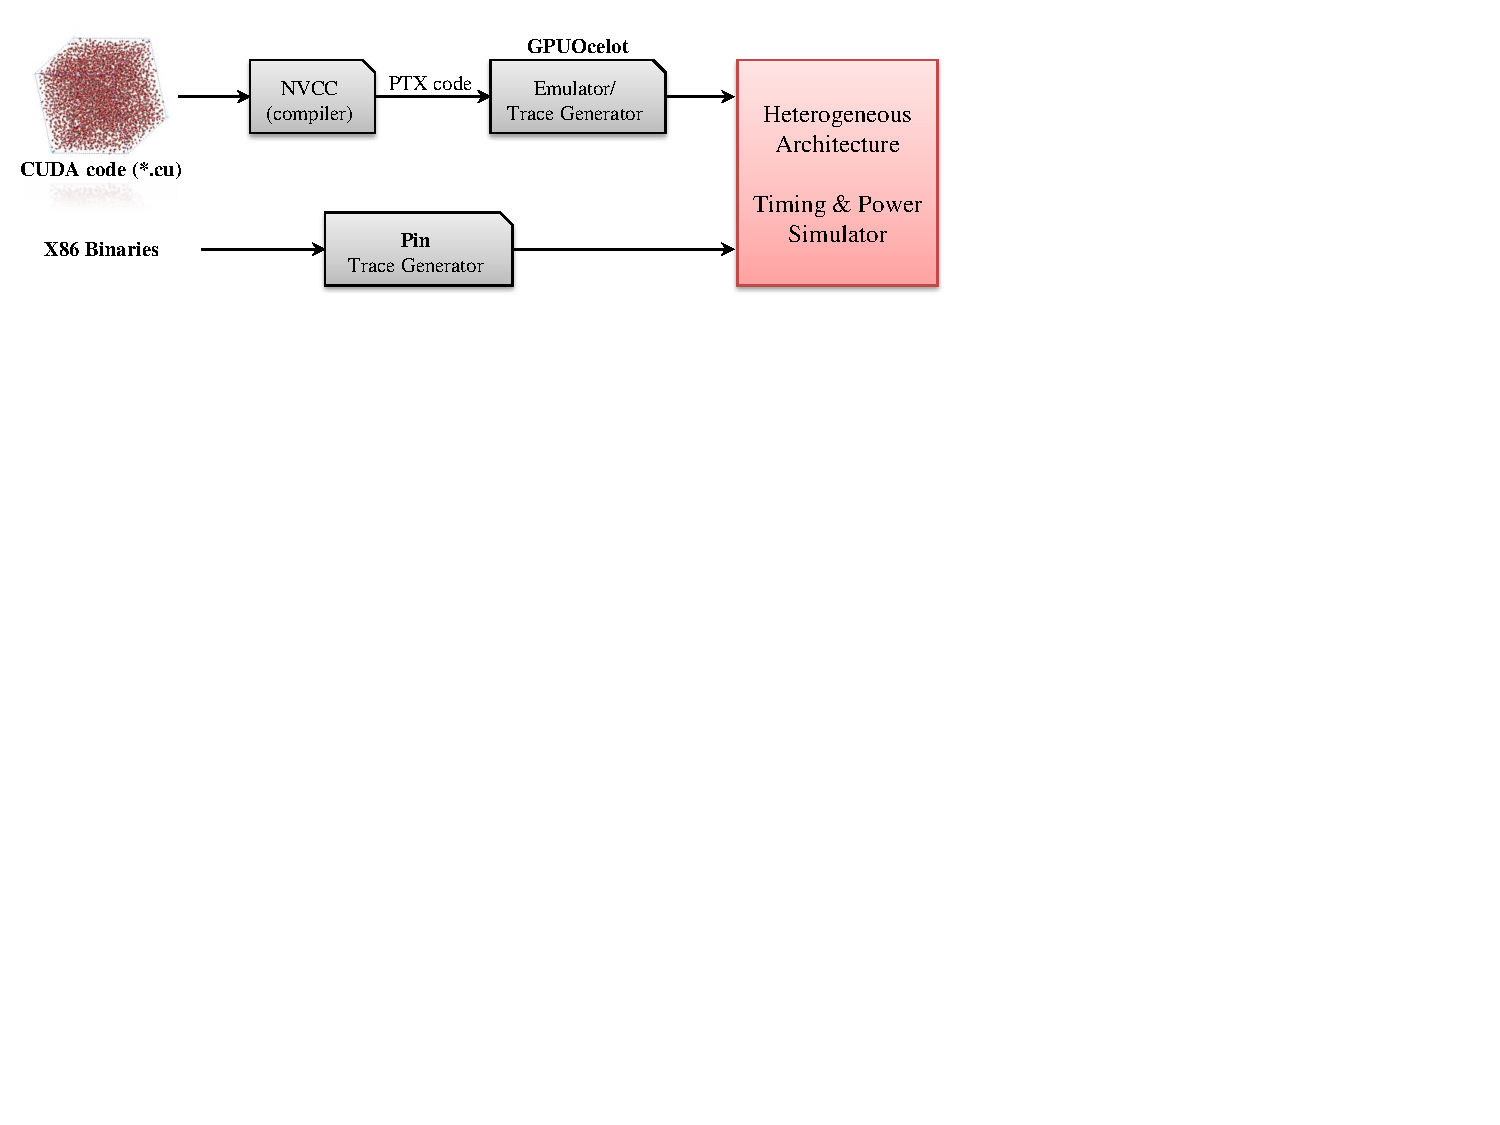
\includegraphics{figs/macsim_overview}
\caption{The overview of MacSim Traces Generation}
\label{fig:overview}
\end{figure*}


%%%%%%%%%%%%%%%%%%%%%%%%%%%%%%%%%%%%%%%%%%%%%%%%%%%%%%%%%%%%%%%%%%%%%%%%
%\section{Trace Generation}
%\label{sec:trace_generation}
%%%%%%%%%%%%%%%%%%%%%%%%%%%%%%%%%%%%%%%%%%%%%%%%%%%%%%%%%%%%%%%%%%%%%%%%



%%%%%%%%%%%%%%%%%%%%%%%%%%%%%%%%%%%%%%%%%%%%%%%%%%%%%%%%%%%%%%%%%%%%%%%%
\section{CPU (x86) Traces}
%%%%%%%%%%%%%%%%%%%%%%%%%%%%%%%%%%%%%%%%%%%%%%%%%%%%%%%%%%%%%%%%%%%%%%%%

\SIM includes a CPU (x86) trace generator which is based on Pin~\cite{pin}, a
binary instrumentation tool. Documentation regarding Pin can be found at
\urlc{http://www.pintool.org}. After installing Pin\footnote{Note that our
trace generator may not be backward/forward compatible with different Pin
versions. Currently, pin 2.12 (version number 56759  )  must be used.}, the x86
trace generator module has to be built. The command for doing so is:


\ignore
		{
		CPU (x86) traces are generated with the aid of Pin~\cite{pin}, a
		binary instrumentation tool.  Documentation regarding Pin can be found 
		here \urlc{http://www.pintool.org}.  We provide
		\cpu trace generator within \SIM repository. After installing
		Pin\footnote{Note that our CPU trace generator may not be
		  backward/forward compatible with the pin version. Currently, pin
		  41150 revision (Jun 07, 2011) must be used.}, we need to build the
		X86 trace generator module (trace\_generator.so), which can be simply
		done with the following commands.
		}



\begin{Verbatim}
cd toos/x86_trace_generator
make
\end{Verbatim}

\noindent This will generate trace\_generator.so in the
tools/x86\_trace\_generator/obj-intel64 directory. x86
traces for \SIM can then be generated by running Pin with the generated module.


\begin{Verbatim}
pin -t trace_generator.so -- $BIN $ARGS (for single-threaded applications)
pin -t trace_generator.so -thread N -- $BIN $ARGS (for multi-threaded applications with N threads)
\end{Verbatim}


The following example shows the generation of traces for an execution of /bin/ls. 

\begin{Verbatim}
pin -t trace_generator.so -- /bin/ls
\end{Verbatim}


\noindent The binary (ls) is actually executed on top of Pin and the
instructions executed by the binary are written to the trace file. The output
on the screen when generating traces for \textit{ls} is shown.

\begin{Verbatim}
pin -t trace_generator.so -- /bin/ls
-> Thread[0->0] begins.
-> Trace Generation Starts at icount 0
dump.txt_0.dump  pin.log  trace_0.raw  trace_generator.o  trace_generator.so  
xed_extractor.o  xed_extractor.so
-> Trace Generation Done at icount 475195
\end{Verbatim}

The trace generator generates two files (in case of a single threaded
application) - Trace.txt and trace\_0.raw, in the current directory.
Section~\ref{sec:traceformat} provides details of the generated files.
It is also possibel to generate traces for a given code section.
Users can add routine call SIM\_BEGIN(1) and SIM\_END(1) in the 
source code to indicate the begin/end point. An example is shown as
follows.

\begin{Verbatim}
pin -t trace\_generator.so -manual 1 -thread N -- $BIN $ARGS (enable user defined annotations) 
\end{Verbatim}

%%%%%%%%%%%%%%%%%%%%%%%%%%%%%%%%%%%%%%%%%%%%%%%%%%%%%%%%%%%%%%%%%%%%%%%%
\section{GPU (PTX) Traces}
\label{sec:gpu_traces}
%%%%%%%%%%%%%%%%%%%%%%%%%%%%%%%%%%%%%%%%%%%%%%%%%%%%%%%%%%%%%%%%%%%%%%%%

GPU (PTX) traces are generated using GPUOcelot~\cite{ocelot}, a dynamic compilation
framework for heterogeneous systems. 


%%%%%%%%%%%%%%%%%%%%%%%%%%%%%%%%%%%%%%%%%%%%%%%%%%%%%%%%%%%%%%%%%%%%%%%%
\subsection{Installing Ocelot}
%%%%%%%%%%%%%%%%%%%%%%%%%%%%%%%%%%%%%%%%%%%%%%%%%%%%%%%%%%%%%%%%%%%%%%%%

Currently Ocelot can be download from github. Ocelot supports up to
CUDA 4.2 so higher CUDA versions need to be compiled with 4.2. 

\begin{Verbatim}
 git clone https://github.com/gtcasl/gpuocelot.git
\end{Verbatim}

A simple guide of compiling Ocelot to generate traces is provided 
at macsim/tools/ocelot\_install\_guide.txt. 
More detailed information is available at Ocelot's homepage. 

\ignore{
Then build Ocelot and the trace generator libraries.

\begin{Verbatim}
cd gpuocelot/ocelot; sudo ./build.py --install
cd gpuocelot/trace-generators; libtoolize; aclocal; autoconf; automake; ./configure; 
make; sudo make install
\end{Verbatim}

All libraries will be installed in the system library path directory
(\Verb+/usr/local/lib+). More detailed instructions for installing
Ocelot are available at Ocelot's Google Code project page.
}


%%%%%%%%%%%%%%%%%%%%%%%%%%%%%%%%%%%%%%%%%%%%%%%%%%%%%%%%%%%%%%%%%%%%%%%%
\subsection{Generating Traces}
%%%%%%%%%%%%%%%%%%%%%%%%%%%%%%%%%%%%%%%%%%%%%%%%%%%%%%%%%%%%%%%%%%%%%%%%

CUDA executables targeted for trace generation must be linked against
libocelot.so and libocelotTrace.so. libocelot.so provides the functionality of
the CUDA runtime library (libcudart.so) and libocelotTrace.so contains the
trace generator for \SIM and tools provided by Ocelot.

To execute a binary linked against libocelot.so a configuration file,
\Verb+configure.ocelot+ (which is in JSON format), is required in the same
directory as the binary. A copy of this file with some default settings can
be obtained from the Ocelot source. To enable trace generation, open your
copy of the configure.ocelot and add the pair \Verb+x86Trace: true+ on a new
line under the trace member as shown below.  Make sure that there is a comma
at the end of each pair that is not the last pair of a member.

\begin{Verbatim}
  trace: {
    database: "traces-ipdom/database.trace",
    memoryChecker: {
      enabled: true,
      checkInitialization: false
    },
    raceDetector: {
      enabled: true,
      ignoreIrrelevantWrites: true
    },
    cacheSimulator: {
      enabled: false,
    },
    branch: false,
    memory: false,
    x86Trace: true
  },
\end{Verbatim}

In addition to editing configure.ocelot, the following four environment
variables have to be set:

\begin{itemize}\itemsep2pt
\item[-] TRACE\_PATH : directory to store generated traces. If not specified, current directory is used by default.
\item[-] TRACE\_NAME : prefix used in the file name for generated traces. If not specified, "Trace" is used by default.
\item[-] KERNEL\_INFO\_PATH : name of file that should contain kernel information (must be specified)
\item[-] COMPUTE\_VERSION : compute capability (default 2.0)
\end{itemize}


Examples for setting up these environment variables are shown below.

\begin{Verbatim}
export TRACE_PATH="/storage/traces/"  # Create a trace directory in the /storage/traces
export KERNEL_INFO_PATH="kernel_info" # kernel_info has the kernel information
export COMPUTE_VERSION="2.0"          # Calculate occupancy based on compute capability 2.0
\end{Verbatim}

On executing the binary of a kernel, an information file and a directory for each
kernel invocation by the binary are generated. These directories contain traces from 
different invocations of the kernel. The directories path are addressed by \Verb+TRACE\_PATH+. 
The kernel information file contains the version of generated traces and path of
each trace configuration file. The trace configuration file contains the number of warps, the
trace version, maximum number of thread blocks that can be assigned to each SM
and the ID, and starting information of each warp. More information regarding
the generated files can be found in Sections~\ref{sec:traceformat} and ~\ref{sec:kern_config}. 

\ignore
		{
		The kernel information file (kernel\_info) should contain the following
		information: kernel name, register usage (per thread), and shared memory usage
		(per thread).


		\begin{Verbatim}
		_Z9Memcpy_SWPfS_i 14 52 
		\end{Verbatim}


		Running CUDA application creates a directory with the kernel name, where traces 
		are generated, and kernel\_config.txt which is a configuration used for MacSim.


		\begin{Verbatim}
		drwxr-xr-x   2 anonymous group 69632 Sep 00 22:03 _Z9Memcpy_SWPfS_i_0
		-rw-r--r--   1 anonymous group    66 Sep 09 22:29 kernel_config.txt
		\end{Verbatim}
		}


%%%%%%%%%%%%%%%%%%%%%%%%%%%%%%%%%%%%%%%%%%%%%%%%%%%%%%%%%%%%%%%%%%%%%%%%
\section{Supporting Other Architectures}
%%%%%%%%%%%%%%%%%%%%%%%%%%%%%%%%%%%%%%%%%%%%%%%%%%%%%%%%%%%%%%%%%%%%%%%%

To support other ISAs such as ARM, a frontend simulator or a
functional emulator is necessary to provide the executed instruction stream. 
Instructions in this stream can be translated by \SIM into
its internal RISC style micro-ops and simulated. Currently, plans for
supporting ARM ISA and OpenGL programs are in progress.


%%%%%%%%%%%%%%%%%%%%%%%%%%%%%%%%%%%%%%%%%%%%%%%%%%%%%%%%%%%%%%%%%%%%%%%%
\section{Trace Formats}
\label{sec:traceformat}
%%%%%%%%%%%%%%%%%%%%%%%%%%%%%%%%%%%%%%%%%%%%%%%%%%%%%%%%%%%%%%%%%%%%%%%%

\paragraph{Note:}

\textit{Although different trace generators use the same data structure for
storing instruction traces, the meaning of some of the members of this
common data structure is different in PTX traces. Note that efforts to
have different data structures for x86 and PTX traces for sake of
extensibility and clarity are underway.}


On a successful trace generation, the x86 trace generator generates a
configuration file called Trace.txt and one Trace\_xx.raw file
(assuming that \Verb+TRACE\_PATH+ was set to "Trace") for each thread
of the application in the output directory. On the other hand, the PTX
trace generator generates a kernel information file and several
directories containing traces of individual kernel invocations. The
directory for each kernel invocation contains a Trace.txt file and one
Trace\_xx.raw file for each warp in the kernel.  Note that in case of
PTX kernels, one trace file is generated for each warp, there are no
per thread trace files. Further details regarding trace generation for
PTX kernels can be found in Section~\ref{sec:ptx_traces}. The purposes
of Trace.txt and Trace\_xx.raw are shown below and their formats are
explained in detail in subsequent sections.


\begin{itemize}\itemsep2pt
\item Trace.txt (info trace): contains information about the generated
  trace files (\#threads, trace type, ...).

\item Trace\_xx.raw (raw trace): contains instruction trace for a
  thread and is generated for each thread.\footnote{In case of GPU, a
    warp is mapped to a \SIM thread, where a warp consists of 32
    threads in CUDA.}
\end{itemize}



%%%%%%%%%%%%%%%%%%%%%%%%%%%%%%%%%%%%%%%%%%%%%%%%%%%%%%%%%%%%%%%%%%%%%%%%
\subsection{Trace.txt}
%%%%%%%%%%%%%%%%%%%%%%%%%%%%%%%%%%%%%%%%%%%%%%%%%%%%%%%%%%%%%%%%%%%%%%%%


\begin{figure*}[htb]
\centering
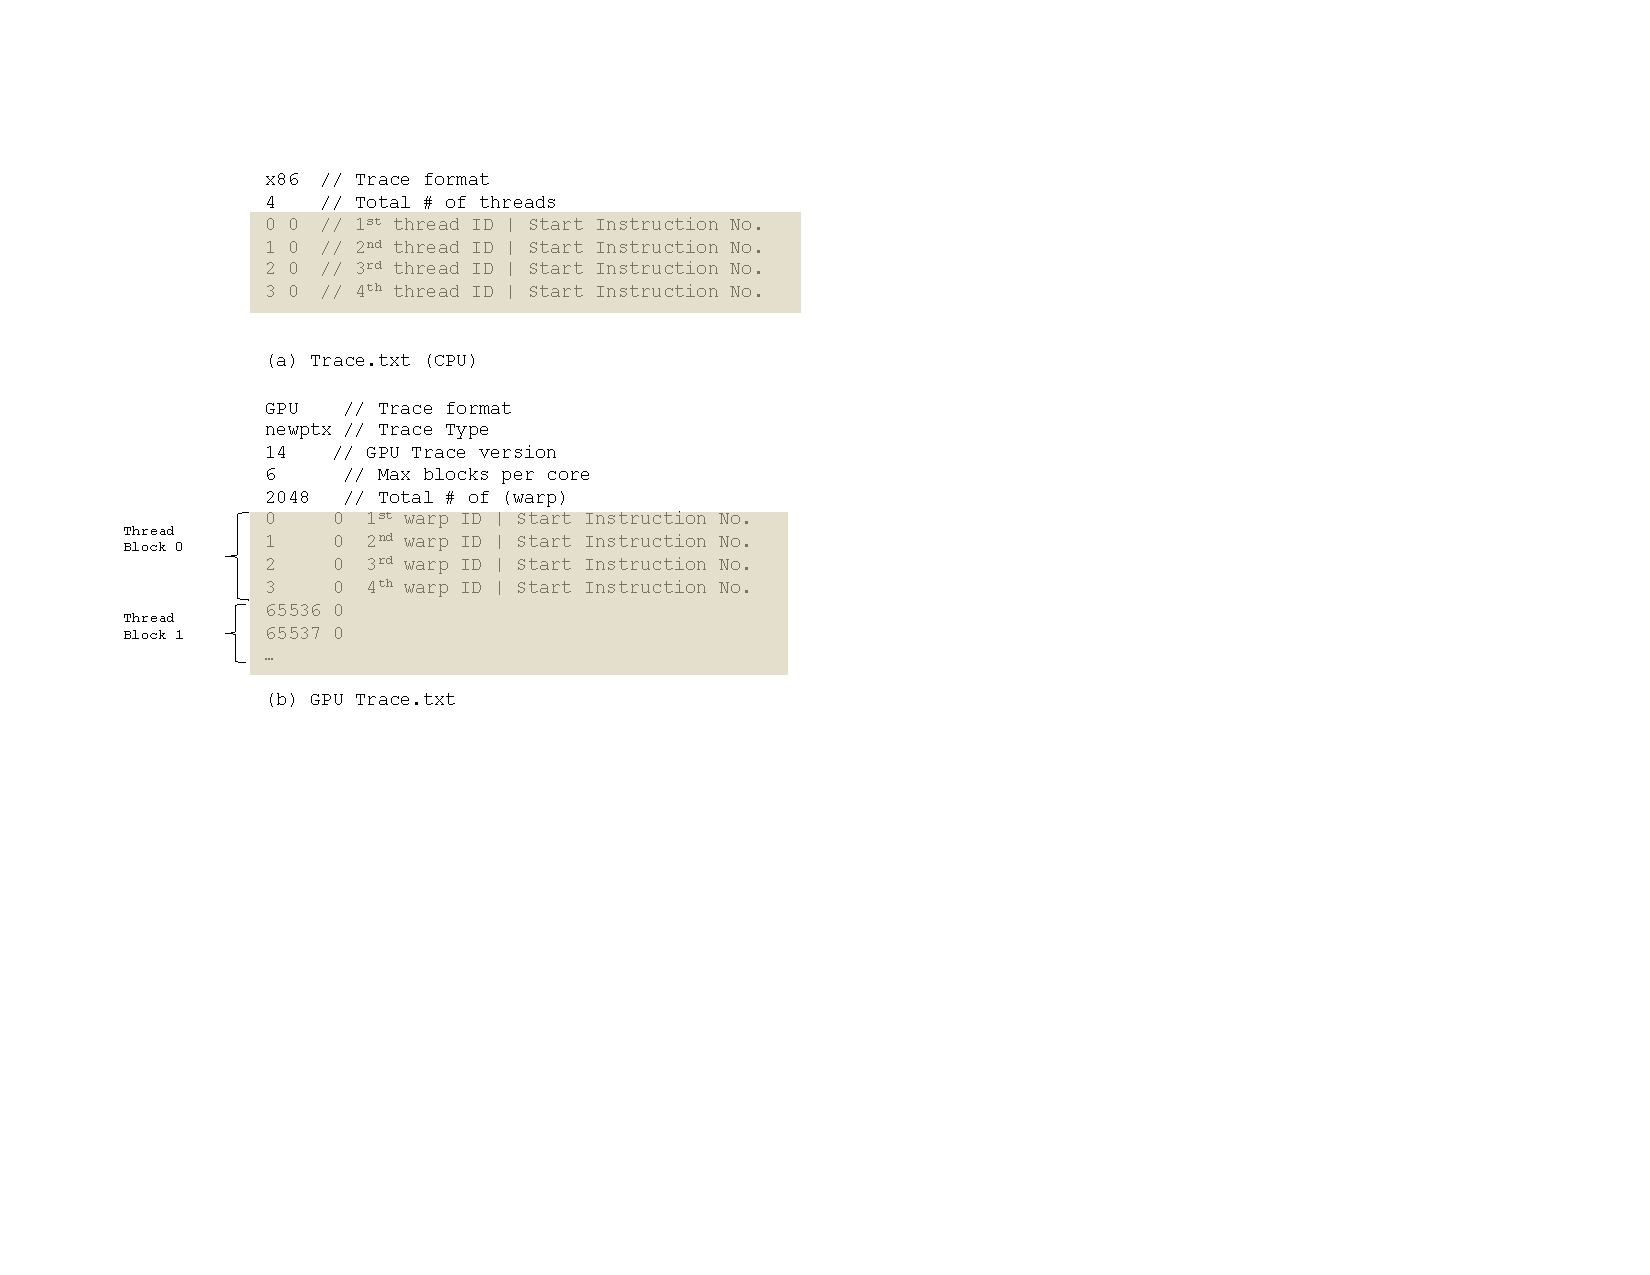
\includegraphics{figs/trace_format}
\caption{Trace.txt format} 
\label{fig:trace_format}
\end{figure*}


Figure~\ref{fig:trace_format}-(a) shows the format of Trace.txt and its CPU and GPU
examples.  As shown in Figure~\ref{fig:trace_format}-(a), the first line in
Trace.txt has different fields from the rest of the lines.

\begin{itemize}\itemsep2pt
\item \#Threads: indicates the number of threads for which traces have
  been generated, and this value is equal to the number of lines in
  the file excluding the first line.
\item Trace Type: indicates whether the generated traces are for an
  x86 application or a PTX kernel.
\item Optional Field(s): currently used for PTX traces only and
  indicates the number of thread blocks that can be assigned to a
  streaming multiprocessor(SM) core (occupancy).
\end{itemize}

From the second line (5th line on GPU format)  onwards, there are two fields in each line:
thread id and start instruction number. For each thread, there is a
Trace\_<thread\_id>.raw file which contains the dynamic instruction
trace for the thread. Finally, start instruction number indicates when
each thread should be started in terms of the number of instructions
simulated for the main thread of the application. In a PTX kernel,
since all warps are ready for execution at the launch of the kernel,
the start instruction number for all threads is zero. On the other
hand, for an x86 application, the start instruction is non-zero for all
threads except thread 0, which is the main (or parent) thread in the
application. This is because in most multi-threaded CPU applications,
main thread (thread id 0) spawns children threads.


In Figure~\ref{fig:trace_format}-(b), the CPU trace has four threads and its
type is set to x86. The ids of the threads are 0-3 with the corresponding trace
files being Trace\_0.raw$-$Trace\_3.raw . Thread 0 is ready at the start of
simulation, while Threads 1, 2 and 3 become ready when Thread 0 has fetched x,
y and z instructions respectively.


In the GPU example, the number of traces files is 2048 since \#Threads
(representing \#Warps in case of GPUs) is 2048.  The optional field indicates
that eight thread blocks can be assigned to a SM core. 

For GPU traces, the id in the file encodes thread block information as
well. The warp id and thread block id can be decoded from this id as follows:

\begin{Verbatim}
warp_id  = id % (1 << 16)
block_id = id / (1 << 16)
\end{Verbatim}

\ignore
		{
		In the GPU trace, thread ID is calculated by thread block ID * 65536 + warp ID (in a block). 
		In the example, warps 0, 1, 2 and 3 are comprised of a thread block, and warps 65536, 65537, 65538
		and 65539 forms another thread block.
		}

%%%%%%%%%%%%%%%%%%%%%%%%%%%%%%%%%%%%%%%%%%%%%%%%%%%%%%%%%%%%%%%%%%%%%%%%
\subsection{Trace\_xx.raw}
%%%%%%%%%%%%%%%%%%%%%%%%%%%%%%%%%%%%%%%%%%%%%%%%%%%%%%%%%%%%%%%%%%%%%%%%

Trace\_xx.raw is generated for each thread/warp and contains the
dynamic instruction trace for the thread/warp in binary
format. The structure/format for encoding instructions is the same in
both x86 and PTX traces and looks like as follows (in order):


%trace format for an instruction in trace_xx.raw

\vspace{0.2in}
\begin{footnotesize}
\begin{tabular}{l c l l}
Type            & Size (Bytes) & Field                     & Description                                            \\ \hline \hline
\Verb+uint8_t+  & 1            & \Verb+m_num_read_regs+    & number of source registers                             \\
\Verb+uint8_t+  & 1            & \Verb+m_num_dest_regs+    & number of destination registers                        \\
\Verb+uint8_t+  & 9            & \Verb+m_src[MAX_SRC_NUM]+ & source register IDs                                    \\
\Verb+uint8_t+  & 6            & \Verb+m_dst[MAX_DST_NUM]+ & destination register IDs                               \\
\Verb+uint8_t+  & 1            & \Verb+m_cf_type+          & branch type                                            \\
\Verb+bool+     & 1            & \Verb+m_has_immediate+    & indicates whether this instruction has immediate field \\
\Verb+uint8_t+  & 1            & \Verb+m_opcode+           & opcode                                                 \\
\Verb+bool+     & 1            & \Verb+m_has_st+           & indicates whether this instruction has store operation \\
\Verb+bool+     & 1            & \Verb+m_is_fp+            & indicates whether this instruction is a FP operation   \\
\Verb+bool+     & 1            & \Verb+m_write_flg+        & write flag                                             \\
\Verb+uint8_t+  & 1            & \Verb+m_num_ld+           & number of load operations                              \\
\Verb+uint8_t+  & 1            & \Verb+m_size+             & instruction size                                       \\
\Verb+uint32_t+ & 4            & \Verb+m_ld_vaddr1+        & load address 1                                         \\
\Verb+uint32_t+ & 4            & \Verb+m_ld_vaddr2+        & load address 2                                         \\
\Verb+uint32_t+ & 4            & \Verb+m_st_vaddr+         & store address                                          \\
\Verb+uint32_t+ & 4            & \Verb+m_instruction_addr+ & PC address                                             \\
\Verb+uint32_t+ & 4            & \Verb+m_branch_target+    & branch target address                                  \\
\Verb+uint8_t+  & 1            & \Verb+m_mem_read_size+    & memory read size                                       \\ 
\Verb+uint8_t+  & 1            & \Verb+m_mem_write_size+   & memory write size                                      \\
\Verb+bool+     & 1            & \Verb+m_rep_dir+          & repetition direction                                   \\
\Verb+bool+     & 1            & \Verb+m_actually_taken+   & indicates whether branch is actually taken             \\
\end{tabular}
\end{footnotesize}
\vspace{0.2in}


Note that the raw trace is compressed with zlib to reduce the sizes of
the generated trace files, and the size of each field is the size
before the compression.


%%%%%%%%%%%%%%%%%%%%%%%%%%%%%%%%%%%%%%%%%%%%%%%%%%%%%%%%%%%%%%%%%%%%%%%%
\subsection{kernel\_config.txt (only for PTX)}
\label{sec:kern_config}
%%%%%%%%%%%%%%%%%%%%%%%%%%%%%%%%%%%%%%%%%%%%%%%%%%%%%%%%%%%%%%%%%%%%%%%%

For PTX traces, as described in Section~\ref{sec:gpu_traces}, a directory is
created for each kernel invocation, where Trace.txt and Trace\_xx.raw are
generated. Since typical GPU applications usually invoke several kernels (or
execute the same kernel repeatedly), PTX traces can have multiple kernel
directories. Thus, in order to simulate all invoked kernels for a GPU
application, the PTX trace generator creates kernel\_config.txt which contains
information of the invoked kernels.


\begin{Verbatim}
Contents of output directory after trace generation

ll /trace/ptx/parboil/bfs

drwxr-xr-x  4  4096 Sep 21 13:21 .
drwxr-xr-x 11  4096 Sep 13 18:02 ..
drwxr-xr-x  2  4096 Apr  7  2011 _Z17BFS_in_GPU_kernelPiS_P4int2S1_S_S_iS_ii_0
drwxr-xr-x  2  4096 Apr  7  2011 _Z26BFS_kernel_multi_blk_inGPUPiS_P4int2S1_S_S_S_S_iiS_S_S__0
-rw-r--r--  1   184 Apr  7  2011 kernel_config.txt

In kernel_config.txt

-1 newptx
/trace/ptx/parboil/bfs/_Z17BFS_in_GPU_kernelPiS_P4int2S1_S_S_iS_ii_0/Trace.txt
/trace/ptx/parboil/bfs/_Z26BFS_kernel_multi_blk_inGPUPiS_P4int2S1_S_S_S_S_iiS_S_S__0/Trace.txt
\end{Verbatim}


As shown above, all the invoked kernels are enumerated in kernel\_config.txt.
The first line indicates that this is a wrapper file which points to (multiple)
trace.txt files, one for each kernel invocation. \SIM reads and simulates the
traces sequentially, one kernel at a time.  In the above example (bfs),
kernel\_config.txt indicates that there are two different kernels in bfs,
each of which was invoked once. When running a GPU simulation, the path to
the kernel\_config.txt file is specified trace\_file\_list
(Section~\ref{sec:run}).  Also, we can simulate specific kernels
by modifying the kernel\_config.txt file.

%%%%%%%%%%%%%%%%%%%%%%%%%%%%%%%%%%%%%%%%%%%%%%%%%%%%%%%%%%%%%%%%%%%%%%%%
\subsection{Translation into micro-ops}
%%%%%%%%%%%%%%%%%%%%%%%%%%%%%%%%%%%%%%%%%%%%%%%%%%%%%%%%%%%%%%%%%%%%%%%%

During simulation, each instruction in a \emph{raw trace} file is
converted into one or more micro-ops internally. \SIM stores such
decoded micro-uops in the \SIM-specific structure shown in
Table~\ref{table:trace_uops}.

\begin{table*}[!htb]
\begin{footnotesize}
\begin{center}
\caption{\SIM-specific data structure for micro-ops.}
\label{table:trace_uops}
\begin{tabular}{|l|l|l|} 
\hline
Type      & Variable                 & Description \\ \hline \hline
uint8\_t  & m\_opcode                & opcode \\ \hline
Uop\_Type & m\_op\_type              & type of operation \\ \hline
Mem\_Type & m\_mem\_type             & type of memory instruction \\ \hline
Cf\_Type  & m\_cf\_type              & type of control flow instruction \\ \hline
Bar\_Type & m\_bar\_type             & type of barrier caused by instruction \\ \hline
uns       &   m\_num\_dest\_regs     & number of destination registers written \\ \hline
uns       &   m\_num\_src\_regs      & number of source registers read \\ \hline
uns       &   m\_mem\_size           & number of bytes read/written by a memory instruction \\ \hline
uns       &   m\_inst\_size          & instruction size \\ \hline
Addr      &   m\_addr                & PC address  \\ \hline
reg\_info\_s&   m\_srcs[MAX\_SRCS]   & source register information \\ \hline
reg\_info\_s&   m\_dests[MAX\_DESTS] & destination register information \\ \hline
Addr      &   m\_va;                 & virtual address \\ \hline
bool      &   m\_actual\_taken       & branch actually taken \\ \hline
Addr      &   m\_target              & branch target address \\ \hline
Addr      &   m\_npc                 & next PC address  \\ \hline
bool      &   m\_pin\_2nd\_mem       & has second memory operation \\ \hline
inst\_info\_s& *m\_info              & pointer to the instruction hash table  \\ \hline
int       &   m\_rep\_uop\_num       & repeated uop number \\ \hline
bool      &   m\_eom                 & end of macro \\ \hline
bool      &   m\_alu\_uop            & ALU uop  \\ \hline
uint32\_t  &   m\_active\_mask       & active mask \\ \hline
uint32\_t  &   m\_taken\_mask        & branch taken mask \\ \hline
Addr      &   m\_reconverge\_addr    & address of reconvergence \\ \hline
bool      &   m\_mul\_mem\_uops      & multiple memory transactions \\ \hline

\end{tabular}
\end{center}
\end{footnotesize}
\end{table*}

\ignore{
		The following shows the data structure for micro-uops. 
		\begin{Verbatim}
		  uint8_t      m_opcode;        /**< opcode */
		  Uop_Type     m_op_type;       /**< type of operation */
		  Mem_Type     m_mem_type;      /**< type of memory instruction */
		  Cf_Type      m_cf_type;       /**< type of control flow instruction */ 
		  Bar_Type     m_bar_type;      /**< type of barrier caused by instruction */
		  uns          m_num_dest_regs; /**< number of destination registers written */
		  uns          m_num_src_regs;  /**< number of source registers read */
		  uns          m_mem_size;      /**< number of bytes read/written by a memory instruction */
		  uns          m_inst_size;     /**< instruction size */
		  Addr         m_addr;          /**< pc address */ 
		  reg_info_s   m_srcs[MAX_SRCS]; /**< source register information */
		  reg_info_s   m_dests[MAX_DESTS]; /**< destination register information */
		  Addr         m_va;            /**< virtual address */
		  bool         m_actual_taken;  /**< branch actually taken */
		  Addr         m_target;        /**< branch target address */
		  Addr         m_npc;           /**< next pc address */ 
		  bool         m_pin_2nd_mem;   /**< has second memory operation */
		  inst_info_s *m_info;          /**< pointer to the instruction hash table */ 
		  int          m_rep_uop_num;   /**< repeated uop number */
		  bool         m_eom;           /**< end of macro */
		  bool         m_alu_uop;       /**< alu uop */ 
		  // GPU simulation
		  uint32_t     m_active_mask;   /**< active mask */
		  uint32_t     m_taken_mask;    /**< branch taken mask */
		  Addr         m_reconverge_addr; /**< address of reconvergence */
		  bool         m_mul_mem_uops;  /**< multiple memory transactions */
		\end{Verbatim}
}

% LocalWords:  GPU PTX gpuocelot

%%%%%%%%%%%%%%%%%%%%%%%%%%%%%%%%%%%%%%%%%%%%%%%%%%%%%%%%%%%%%%%%%%%%%%%%%%%%%%%%%%%%%%

\ignore
		{
		\begin{table*}[htb]
		\begin{footnotesize}
		\begin{center}
		\caption{MacSim trace format.}
		\label{table:trace_format}
		\begin{tabular}{|l|l|} 
		\hline
		Type               & Description \\ \hline 
		uint8\_t           & number of source registers \\ \hline
		uint8\_t           & number of destination registers \\ \hline
		uint8\_t[9]        & source register IDs \\ \hline
		uint8\_t[6]        & destination register IDs \\ \hline
		uint8\_t           & branch type \\ \hline
		bool               & indicates whether this instruction has immediate field \\ \hline
		uint8\_t           & opcode \\ \hline
		bool               & indicates whether this instruction has store operation \\ \hline
		bool               & indicates whether this instruction is FP operation \\ \hline
		bool               & write flag \\ \hline
		uint8\_t           & number of load operations \\ \hline
		uint8\_t           & instruction size \\ \hline
		uint32\_t          & load address 1 \\ \hline
		uint32\_t          & load address 2 \\ \hline
		uint32\_t          & store address \\ \hline
		uint32\_t          & PC address \\ \hline
		uint32\_t          & branch target address \\ \hline
		uint32\_t          & memory read size \\ \hline
		uint8\_t           & memory write size \\ \hline
		uint8\_t           & repetition direction  \\ \hline
		uint8\_t           & indicates whether branch is actually taken \\ \hline

		\end{tabular}
		\end{center}
		\end{footnotesize}
		\end{table*}
		}

\ignore
		{
		\begin{table*}[htb]
		\begin{footnotesize}
		\begin{center}
		\caption{MacSim trace format.}
		\label{table:trace_format}
		\begin{tabular}{|l|l|l|l|l|l|l|l|l|l|l|l|l|l|l|l|} 
		\hline
		nSR & nDR & SR\_IDs & DR\_IDs & BrType & bImm & Opcode & bStore & bFP & WF & nLD  \\ \hline \hline
		InstSize & LAddr\_1 & LAddr\_2 & SAddr & PCAddr & BrAddr & MemRSize & MemWSize & RepDir & BrActT & \\ \hline
		\end{tabular}
		\end{center}
		\end{footnotesize}
		\end{table*}

		Tables~\ref{table:trace_format} and ~\ref{table:trace_desc} show the trace
		format for each instruction and the description of each field, respectively.
		}

 

/*
Copyright (c) <2012>, <Georgia Institute of Technology> All rights reserved.

Redistribution and use in source and binary forms, with or without modification, are permitted 
provided that the following conditions are met:

Redistributions of source code must retain the above copyright notice, this list of conditions 
and the following disclaimer.

Redistributions in binary form must reproduce the above copyright notice, this list of 
conditions and the following disclaimer in the documentation and/or other materials provided 
with the distribution.

Neither the name of the <Georgia Institue of Technology> nor the names of its contributors 
may be used to endorse or promote products derived from this software without specific prior 
written permission.

THIS SOFTWARE IS PROVIDED BY THE COPYRIGHT HOLDERS AND CONTRIBUTORS "AS IS" AND ANY EXPRESS OR 
IMPLIED WARRANTIES, INCLUDING, BUT NOT LIMITED TO, THE IMPLIED WARRANTIES OF MERCHANTABILITY 
AND FITNESS FOR A PARTICULAR PURPOSE ARE DISCLAIMED. IN NO EVENT SHALL THE COPYRIGHT HOLDER OR 
CONTRIBUTORS BE LIABLE FOR ANY DIRECT, INDIRECT, INCIDENTAL, SPECIAL, EXEMPLARY, OR 
CONSEQUENTIAL DAMAGES (INCLUDING, BUT NOT LIMITED TO, PROCUREMENT OF SUBSTITUTE GOODS OR 
SERVICES; LOSS OF USE, DATA, OR PROFITS; OR BUSINESS INTERRUPTION) HOWEVER CAUSED AND ON ANY 
THEORY OF LIABILITY, WHETHER IN CONTRACT, STRICT LIABILITY, OR TORT (INCLUDING NEGLIGENCE OR 
OTHERWISE) ARISING IN ANY WAY OUT OF THE USE OF THIS SOFTWARE, EVEN IF ADVISED OF THE 
POSSIBILITY OF SUCH DAMAGE.
*/



param<ENABLE_INST_COUNT, enable_inst_count, bool, false>
param<ENABLE_REUSE_DIST, enable_reuse_dist, bool, false>
param<ENABLE_COUNT_STATIC_PC, enable_count_static_pc, bool, false>



%%%%%%%%%%%%%%%%%%%%%%%%%%%%%%%%%%%%%%%%%%%%%%%%%%%%%%%%%%%%%%%%%%%%%%%%
\chapter{Simulation Statistics}
\label{sec:stat}
%%%%%%%%%%%%%%%%%%%%%%%%%%%%%%%%%%%%%%%%%%%%%%%%%%%%%%%%%%%%%%%%%%%%%%%%

A simple framework for collecting statistics (hereafter referred to as stats)
during simulation is provided.  Stats can be either global (includes
data from all cores) or per core.

%%%%%%%%%%%%%%%%%%%%%%%%%%%%%%%%%%%%%%%%%%%%%%%%%%%%%%%%%%%%%%%%%%%%%%%%
\section{Stat Types}
%%%%%%%%%%%%%%%%%%%%%%%%%%%%%%%%%%%%%%%%%%%%%%%%%%%%%%%%%%%%%%%%%%%%%%%%

The following stat types are supported:

\begin{description}

  \item [COUNT] for counting the number of occurrences of an event. (Eg. number
  of cache hits)

  \item [RATIO] for calculating the ratio of number of occurrences of one event
  over another. (Eg. (number of cache hits / number of cache accesses) i.e.,
  cache hit ratio )

  \item [DIST]  for calculating the proportion of each event in a group of
  events. (Eg. If the user wants to know what percent of L1 data cache accesses 
  (in a 2-level hierarchy) resulted in L1 hits, L2 hits or memory accesses, then the
  user should define a distribution consisting on three events - L1 hits,
  L2 hits and L2 misses  - and update the
 counter for each event separately) 

\end{description}

Note that a simulation will output two values for each stat. First one is the
raw value i.e. the number of occurrences of the event associated with the
stat and the second value is the value calculated based on the type
of the stat.


%%%%%%%%%%%%%%%%%%%%%%%%%%%%%%%%%%%%%%%%%%%%%%%%%%%%%%%%%%%%%%%%%%%%%%%%
\section{Adding a new stat}
%%%%%%%%%%%%%%%%%%%%%%%%%%%%%%%%%%%%%%%%%%%%%%%%%%%%%%%%%%%%%%%%%%%%%%%%

New stats can be defined by adding DEF\_STAT statements to any of the
\textit{*.stat.def} files in the \textit{def/} directory or by creating a
\textit{.stat.def} file including the definitions in the same
directory.  To define a per core statistic specify PER\_CORE at the
end of each DEF\_STAT statement. Below is a description and an example of 
defining stats for different types of stats.


\begin{description}

\item[COUNT Stat:] \Verb+ +
\par \Verb+DEF_STAT(STAT_NAME, COUNT, NO_RATIO [, PER_CORE])+
\par Eg: 
\begin{Verbatim}
DEF_STAT(INST_COUNT_TOT, COUNT, NO_RATIO)
DEF_STAT(INST_COUNT, COUNT, NO_RATIO, PER_CORE)
\end{Verbatim}

\item[RATIO Stat:] \Verb+ +
\par \Verb+DEF_STAT(STAT_NAME, RATIO, BASE_STAT_NAME [, PER_CORE])+
\par In addition to defining the RATIO stat itself, a base stat of type COUNT has to
be defined as well. The value of the base stat is used as the denominator in
calculating the ratio. 
\par Eg: 
\begin{Verbatim}
DEF_STAT(DISPATCHED_INST, COUNT, NO_RATIO)
DEF_STAT(DISPATCH_WAIT, RATIO, DISPATCHED_INST)
\end{Verbatim}

\item[DIST Stat:] \Verb+ +
\begin{Verbatim}
DEF_STAT(STAT_NAME_START, DIST, NO_RATIO [, PER_CORE])
DEF_STAT(STAT_NAME, COUNT, NO_RATIO [, PER_CORE])*
DEF_STAT(STAT_NAME_END, DIST, NO_RATIO [, PER_CORE])
\end{Verbatim}
\par The definition of a DIST stat requires at least two stats.
Eg: 
\begin{Verbatim}
DEF_STAT(SCHED_FAILED_REASON_SUCCESS, DIST, NO_RATIO, PER_CORE)
DEF_STAT(SCHED_FAILED_OPERANDS_NOT_READY, COUNT, NO_RATIO, PER_CORE)
DEF_STAT(SCHED_FAILED_NO_PORTS, DIST, NO_RATIO, PER_CORE)
\end{Verbatim}

\end{description}


%%%%%%%%%%%%%%%%%%%%%%%%%%%%%%%%%%%%%%%%%%%%%%%%%%%%%%%%%%%%%%%%%%%%%%%%
\section{Updating Stats}
%%%%%%%%%%%%%%%%%%%%%%%%%%%%%%%%%%%%%%%%%%%%%%%%%%%%%%%%%%%%%%%%%%%%%%%%
  
Macros are provided to update the value of stats. STAT\_EVENT and
STAT\_EVENT\_M increment and decrement the value of a global stat by 1 and take
the name of the stat to be updated as their argument.  STAT\_EVENT\_N is used
to increment the value of a global stat by more than than 1. It takes the name
of the stat to be incremented and the value to be added as its arguments.
STAT\_CORE\_EVENT and STAT\_CORE\_EVENT\_M increment and decrement the value of
a per core stat by 1. These take core id and the name of the stat to be
incremented/decremented as their parameters. For example,

\begin{tabular}{ll}
 \Verb+STAT_EVENT(INST_COUNT_TOT);+ & \Verb+// increments global stat INST_COUNT_STAT by 1+ \\
 \Verb+STAT_EVENT_N(INST_COUNT_TOT, 2); + & \Verb+// increments global stat INST_COUNT_STAT by 2+ \\
 \Verb+STAT_EVENT_M(INST_COUNT_TOT);+ & \Verb+// decrements global stat INST_COUNT_STAT by 1+ \\
 \Verb+STAT_CORE_EVENT(0, INST_COUNT); + & \Verb+// increments stat INST_COUNT for core 0 by 1+ 
\end{tabular}

%%%%%%%%%%%%%%%%%%%%%%%%%%%%%%%%%%%%%%%%%%%%%%%%%%%%%%%%%%%%%%%%%%%%%%%%
\section{Simulation output}
%%%%%%%%%%%%%%%%%%%%%%%%%%%%%%%%%%%%%%%%%%%%%%%%%%%%%%%%%%%%%%%%%%%%%%%%

At the end of a simulation several files with the extension stat.out are
generated, these files include the stat values at the end of the
simulation. As mentioned, for each stat two values are generated, one is the
raw stat value and other is a value calculated based on the type of the
stat. For simulations with multiple applications, multiple sets of stat files
are generated. Each simulated application is assigned an integer id (these ids
are assigned according to the order in which the applications appear in the
trace\_file\_list), when an application terminates (for the first time,
note that applications may be repeated), stat files suffixed with the the
id of the application, i.e.  *.stat.out.<appl\_id>, are generated. These
stat files contain the value of the stats until that point in the
simulation. At the end of the simulation, *.stat.out files are generated as
usual.



%%%%%%%%%%%%%%%%%%%%%%%%%%%%%%%%%%%%%%%%%%%%%%%%%%%%%%%%%%%%%%%%%%%%%%%%
\section{Important Stats}
%%%%%%%%%%%%%%%%%%%%%%%%%%%%%%%%%%%%%%%%%%%%%%%%%%%%%%%%%%%%%%%%%%%%%%%%
In table \ref{table:stats} some important stats are listed. 

\begin{table}[htb]
\begin{footnotesize}
\begin{center}
\caption{Some important Stats} 
\label{table:stats}
\begin{tabular}{|l||l|c|l|}
\hline 
INST\_COUNT\_TOT            & \# of instructions                                    &      & general.stat.out \\ \hline 
INST\_COUNT\_CORE\_[0-11]   & \# of instructions in only the specificed core [0-11] & core & general.stat.out \\ \hline 
CYC\_COUNT\_TOT             & \# of times simulator cycle is called
(Not total cycle)                                       &      & general.stat.out \\ \hline 
CYC\_COUNT\_CORE\_[0-11]    & simulated cycles in only the specificed core [0-11]   &      & general.stat.out \\ \hline 
CYC\_COUNT\_X86             & simulated cycles for x86 only
&      & general.stat.out \\ \hline \hline 
CYC\_COUNT\_PTX             & simulated cycles for ptx only &      & general.stat.out \\ \hline 
EXE\_Time &  Actual simulation time on the host machine  &  &
general.stat.out \\ \hline \hline 
%FP_OPS_TOT            & \# of fp instructions                                 &   inst.stat.out   &                  \\ \hline 
 %                           & \# of int instructions                                &      &                  \\ \hline 
  %                          & \# of load instructions                               &      &                  \\ \hline  
   %                         & \# of store instructions                              &      &                  \\ \hline  
BP\_ON\_PATH\_CORRECT       & \# of correctly predicted branches (DIST)             & core & bp.stat.def      \\ \hline  
BP\_ON\_PATH\_MISPREDICT    & \# of mis-predicted branches (DIST)                   & core & bp.stat.def      \\ \hline  
BP\_ON\_PATH\_MISFETCHT     & \# of mis-fetch branches (BTB MISS)(DIST)             & core & bp.stat.def      \\ \hline  
ICACHE\_HIT, ICACHE\_MISS   & \# of I-cache hitt,miss (DIST)                        &      & memory.stat.def  \\ \hline  
L[1-3]\_HIT\_CPU            & \# of l[1-3]cache hits from CPU                       &      & memory.stat.def  \\ \hline 
L[1-3]\_HIT\_GPU            & \# of l[1-3]cache hits from GPU                       &      & memory.stat.def  \\ \hline 
L[1-3]\_MISS\_CPU           & \# of l[1-3]cache misses from CPU                     &      & memory.stat.def  \\ \hline 
L[1-3]\_MISS\_GPU           & \# of l[1-3]cache misses from GPU                     &      & memory.stat.def  \\ \hline  \hline 
AVG\_MEMORY\_LATENCY        & average memory latency                                &      & memory.stat.def  \\ \hline \hline 
TOTAL\_DRAM                 & \# of DRAM accesses                                   &      & memory.stat.def  \\ \hline  
TOTAL\_DRAM\_READ           & \# of DRAM reads                                      &      & memory.stat.def  \\ \hline  
TOTAL\_DRAM\_WB             & \# of DRAM write backs                                &      & memory.stat.def  \\ \hline  
%                            & \# of register reads                                  &      &                  \\ \hline  
 %                           & \# of register writes                                 &      &                  \\ \hline   \hline 
COAL\_INST, UNCOAL\_INST    & coalesced/uncoalesced mem requests (DIST)             &      & memory.stat.def  \\ \hline 




\end{tabular}
\end{center}
\end{footnotesize}
\end{table} 



\chapter{\SIM Directory Structure and Source Code}


\section{Directory Structure}

The top-level source directory of \SIM contains several directories. The list of directories is following:

\vspace{0.2in}
\noindent
\begin{footnotesize}
\begin{tabular}{ll}
\Verb+bin/+     & Build output directory                                                                                                                    \\
\Verb+def/+     & Contains definitions of parameters (see Sections~\ref{sec:run} and~\ref{sec:knob}) and events for statistics (see Section~\ref{sec:stat}) \\
\Verb+doc/+     & Contains \SIM documentation.                                                                                                              \\
\Verb+params/+  & Contains sample parameter (see Sections~\ref{sec:run} and~\ref{sec:knob}) configuration files.                                            \\
\Verb+scripts/+ & Contains scripts used in build of \SIM.                                                                                                                                           \\
\Verb+src/+     & Contains \SIM source files (.cc and .h files).                                                                                                                                           \\
\Verb+tools/+   & Contains x86 trace generator and trace reader.                                                                                                                                           \\
\end{tabular}
\end{footnotesize}

\vspace{0.2in}
Table~\ref{table:file_list} shows the list of source file and the purpose/content of
each file.

\begin{table}[htb]
\begin{footnotesize}
\begin{center}
\caption{Source files and their purpose/content}
\label{table:file_list}
\begin{tabular}{|c||c|}
\hline 
File(s)                                                      & Purpose                            \\ \hline
frontend.cc/h, fetch\_factory.cc/h, bp*.cc/h                 & Fetch stage                        \\ \hline 
allocate*.cc/h, rob*.cc/h, map.cc/h                          & Decode and Allocate stages         \\ \hline
schedule*.cc/h                                               & Schedule stage                     \\ \hline 
exec.cc/h                                                    & Execution stage                    \\ \hline 
retire.cc/h                                                  & Retire stage                       \\ \hline       
port.cc/h, cache.cc/h dram.cc/h, memory*.cc/h, 				 & Memory system 					  \\ 
memreq\_info.cc/h, readonly\_cache.cc/h, 					 & 									  \\ 
sw\_managed\_cache.cc/h                                      & 				                      \\ \hline 
pref*.cc/h                                                   & Prefetchers                        \\ \hline
trace\_read.cc/h inst\_info.h                                & Reading traces                     \\ \hline
core.cc/h                                                    & Class representing a core being simulated \\ \hline
process\_manager.cc/h                                        & Process Manager/thread scheduler   \\ \hline 
uop.cc/h                                                     & Uop structure and related enums    \\ \hline
macsim.cc/h					                                 & Class containing pointers to the simulated cores, NoC, \\
                                                             & memory system, knobs and other objects \\ \hline
knob.cc/h                                                    & Classes for supporting knobs       \\ \hline
statistics.cc/h                                              & Classes for supporting knobs       \\ \hline
factory\_class.cc/h                                          & Implementation of different factory classes                          \\ \hline
bug\_detector.cc/h                                           & Class useful for debugging forward progress errors happen             \\ \hline
utils.cc/h                                                   & Utility classes and functions      \\ \hline
debug\_macros.h                                              & Macros for debugging               \\ \hline
assert\_macros.h                                             & Macros for assert statements with debug information                  \\ \hline
global*.h                                                    & Forward declarations and typedefs  \\ \hline

\end{tabular}
\end{center}
\end{footnotesize}
\end{table}



\ignore
{
\begin{table}[htb]
\begin{footnotesize}
\begin{center}
\caption{Pipeline stage and the corresponding source files.}
\label{table:pipeline}
\begin{tabular}{|c||c|}
\hline 
pipeline stage         & file names                                             \\ \hline \hline 
main simulator         & macsim.cc, core.cc                                     \\ \hline 
fetch stage            & frontend.cc, fetch\_factory.cc, bp.cc, bp\_*.cc        \\ \hline 
decode stage           & allocate.cc                                            \\ \hline 
allocate stage         & allocate.cc, allocate\_*.cc, rob.cc, rob\_*.cc, map.cc \\ \hline 
schedule stage         & schedule.cc, schedule\_*.cc                            \\ \hline 
execution stage        & exec.cc                                                \\ \hline 
retire stage           & retire.cc                                              \\ \hline 
memory system          & port.cc, cache.cc *\_cache.cc, dram.cc, memory.cc      \\ \hline \hline
other supporting files & statistics.cc, bug\_detector.cc                        \\ \hline \hline 
process manager        & process\_manager.cc                                    \\ \hline 
\end{tabular}
\end{center}
\end{footnotesize}
\end{table}
}



%

%%%%%%%%%%%%%%%%%%%%%%%%%%%%%%%%%%%%%%%%%%%%%%%%%%%%%%%%%%%%%%%%%%%%%%%%
\chapter{Pipeline Stages in \SIM}
\label{sec:pipeline}
%%%%%%%%%%%%%%%%%%%%%%%%%%%%%%%%%%%%%%%%%%%%%%%%%%%%%%%%%%%%%%%%%%%%%%%%

\SIM implements a five stage pipelined processor whose pipeline depth can 
be varied using knobs. The stages are - Fetch, Decode, Schedule and Execute (includes
Memory) and Retire. This chapter describes the basic feature of each
stage.

%%%%%%%%%%%%%%%%%%%%%%%%%%%%%%%%%%%%%%%%%%%%%%%%%%%%%%%%%%%%%%%%%%%%%%%%
\section{Fetch Stage}
%%%%%%%%%%%%%%%%%%%%%%%%%%%%%%%%%%%%%%%%%%%%%%%%%%%%%%%%%%%%%%%%%%%%%%%%
This stage models the instruction fetch stage, its main tasks
are as follows:

\begin{enumerate}

\item Determine the thread from which instructions will be fetched next \footnote{for
    processors that are not multi-threaded, the same thread is selected
    always}, this involves checking whether a thread can actually fetch a new
	instruction or not

\item Access I-cache \footnote {when there is an I-cache miss, the front-end cannot fetch
    instructions for the selected thread}

\item Read a uop from trace (call {\textit get\_uops\_from\_traces()})

\item BTB access and branch prediction.
  \begin{itemize}
   \item Different branch predictors are implemented using the \textit{bp\_factory}
   \item Type of branch predictor to be used is set using the bp\_dir\_mech knob
  \end{itemize}

\item Send uop to queue meant for modeling the depth of the processor
  front-end.
  \begin{itemize}
   \item Depth of the front-end stage is set using one of the
	  \Verb+fetch_latency+ knobs.\footnote{There is one knob for each core
		type, small, medium, and large}
   \item Different thread fetch policies can be implemented. More details in
		Section~\ref{sec:modify:fetch}.
   \item Default fetch policy is \Verb+round-robin+ and \Verb+fetch_policy+ knob 
		will specify the policy to be used.
  \end{itemize}
  
\end{enumerate}


\ignore
		{ Different fetch polices are implemented using virtual
		  function.  {\textit fetch\_factory} function sets different {\textit
		  frontend\_c}.  Currently, a thread is selected based on the
		  round-robin policy. If the next thread is blocked to fetch, the next
		  candidate is selected based on the round-robin policy.  Different
		  branch predictor policies are also implemented and it is also set by
		  {\textit bp\_factory}. The type of branch predictor or the fetch
		  polices are set by knobs.}


%%%%%%%%%%%%%%%%%%%%%%%%%%%%%%%%%%%%%%%%%%%%%%%%%%%%%%%%%%%%%%%%%%%%%%%%
\subsection{Reading Traces}
%%%%%%%%%%%%%%%%%%%%%%%%%%%%%%%%%%%%%%%%%%%%%%%%%%%%%%%%%%%%%%%%%%%%%%%%

Reading of traces is mainly performed in \Verb+trace_read.cc+. The
main function of this step during simulation is to read a macro
instruction from the trace file and convert it into a sequence of one
or more micro-ops (uops). A simple decoding algorithm is used for
generating uops. To improve the speed of simulation, decoded uops are
stored in a hash table for reuse when the same static instruction is
encountered again during simulation. Note that to obtain dynamic
information such as addresses accessed, uops must be decoded partially
every time.

\ignore 
	  { The main task of trace read is reading an macro instruction from
	  trace file and convert it to uops.  A simple decoding algorithm is used to
	  generate micro uops.  To improve the simulation speed, decoded uops are
	  stored in a hash table.  Which trace file to open is decided in
	  process\_manager.cc }

%%%%%%%%%%%%%%%%%%%%%%%%%%%%%%%%%%%%%%%%%%%%%%%%%%%%%%%%%%%%%%%%%%%%%%%%
\section{Decode and  Allocate Stage}
%%%%%%%%%%%%%%%%%%%%%%%%%%%%%%%%%%%%%%%%%%%%%%%%%%%%%%%%%%%%%%%%%%%%%%%%

\ignore
	  {
	  \todo{Decode is done in frontend.cc!}
	  \todo{according to code, frontend\_q latency = fetch\_latency + alloc\_latency}
	  \todo{according to code, alloc\_q latency = alloc\_to\_exec\_latency}
	  }

In this stage the resource requirement for each uop is calculated and space is
allocated in the required structures for the uop. At the end of this stage, each
uop occupies an entry in ROB and one of the issues queues - general purpose
(integer), floating point or memory. Depending on the knob values, there could
be a unified issue queue or distributed issue queues. For conditional branches
with BTB misses, the branch target is resolved in this stage as well.

%%%%%%%%%%%%%%%%%%%%%%%%%%%%%%%%%%%%%%%%%%%%%%%%%%%%%%%%%%%%%%%%%%%%%%%%
\section{Schedule Stage}
%%%%%%%%%%%%%%%%%%%%%%%%%%%%%%%%%%%%%%%%%%%%%%%%%%%%%%%%%%%%%%%%%%%%%%%%

The schedule stage implements the instruction scheduling logic. Currently
in-order, out-of-order and GPU schedulers are supported. The GPU scheduler
issues uops from the same warp/SIMD thread in order, but uops from different
warps/SIMD threads can be issued out of order in comparison to the order in
which they were dispatched. Before executing an uop the instruction scheduler
first checks for the availability of source operands, and then for the
availability of ports (functional units) for uop execution. 

\ignore
		{ The scheduler stage implements scheduling logic. Currently it supports
		in-order, out-of-order, and GPU scheduling mechanism.  First, it checks the
		source code availability and then functional unit availability-by checking
		ports.  The scheduler is implemented in a virtual function so different
		scheduling policies overload the scheduling functions.}

%%%%%%%%%%%%%%%%%%%%%%%%%%%%%%%%%%%%%%%%%%%%%%%%%%%%%%%%%%%%%%%%%%%%%%%%
\section{Execution Stage}
%%%%%%%%%%%%%%%%%%%%%%%%%%%%%%%%%%%%%%%%%%%%%%%%%%%%%%%%%%%%%%%%%%%%%%%%

In this stage, all instructions - both non-memory and memory - are executed.
The member variable \textit{m\_done\_cycle} of the uop structure indicates the
cycle in which the uop will complete. The following tasks are executed in this
stage:

\begin{itemize}

\item For non-memory uops, the latency of the the instruction is determined, an
	  execution port is marked as in use and the \textit{m\_done\_cycle} of the uop
	  is set. The latencies of uops are defined in the file
	  \textit{../def/uoplatency\_ptx.def} which gets included during the compilation
	  of the \SIM binary. 
	  
\item Branch instructions are resolved in this stage.

\item For memory uops, D-cache \footnote{or the appropriate memory structure such as
    Constant cache, Shared Memory, ...} is accessed and an execution port is
	marked as in use. If a D-cache port is available, then the port is marked as
	used, however, if a port is unavailable, the execution of the uop is attempted
	again later on. On D-cache hit, the \textit{m\_done\_cycle} of the uop is set.
	Handling of D-cache misses is explained in Section~\ref{sec:memory}.

\item Uncoalesced memory instructions result in multiple accesses to the the D-cache.

\ignore
		{ \item \todo[inline]{The number of function units can be specified via
		these knobs for the core type being used - \textit{int\_sched\_rate,
		mem\_sched\_rate, fp\_sched\_rate} - code does not use these in that
		sense}.  }

\end{itemize}

%%%%%%%%%%%%%%%%%%%%%%%%%%%%%%%%%%%%%%%%%%%%%%%%%%%%%%%%%%%%%%%%%%%%%%%%
\section{Retire Stage}
%%%%%%%%%%%%%%%%%%%%%%%%%%%%%%%%%%%%%%%%%%%%%%%%%%%%%%%%%%%%%%%%%%%%%%%%

This stage handles the in-order retirement of uops. Also, memory allocated to a uop
is freed (returned to memory pool). This stage also checks of completion of
warps, blocks, kernels ,and entire application and triggers the
repetition of applications if the knob for repetition is set. (\textit{repeat\_trace})

\ignore
		{
		\todo[inline]{At present, there are no rename and writeback stages in MacSim since
		they are not necessary to support correct and accurate simulation. MacSim
		enforces RAW dependencies, while WAR and WAW dependences can be ignored by
		assuming that once a instruction completes, its results are available for
		dependent instructions without being overwritten.}
		}

\ignore 
		  {
		  %%%%%%%%%%%%%%%%%%%%%%%%%%%%%%%%%%%%%%%%%%%%%%%%%%%%%%%%%%%%%%%%%%%%%%%%
		  \section{Queues}
		  %%%%%%%%%%%%%%%%%%%%%%%%%%%%%%%%%%%%%%%%%%%%%%%%%%%%%%%%%%%%%%%%%%%%%%%%

		  frontend queue
		  ia queue
		  rob
		  scheduler
		  }


% LocalWords:  doxygen frontend bp uops  GPU uop dcache uncoalesced BTB fe mem
% LocalWords:  sched fp icache ptx

%%%%%%%%%%%%%%%%%%%%%%%%%%%%%%%%%%%%%%%%%%%%%%%%%%%%%%%%%%%%%%%%%%%%%%%%
\chapter{The Memory System}
\label{sec:memory}
%%%%%%%%%%%%%%%%%%%%%%%%%%%%%%%%%%%%%%%%%%%%%%%%%%%%%%%%%%%%%%%%%%%%%%%%
In this section \SIM memory system is explained. First, we describe caches,
then memory system hierarchy and organization. Next, configuring different
memory systems are investigated. Finally, DRAM module is explained.

%%%%%%%%%%%%%%%%%%%%%%%%%%%%%%%%%%%%%%%%%%%%%%%%%%%%%%%%%%%%%%%%%%%%%%%%
\section{Caches}
%%%%%%%%%%%%%%%%%%%%%%%%%%%%%%%%%%%%%%%%%%%%%%%%%%%%%%%%%%%%%%%%%%%%%%%%

Each cache structure consists of the cache storage (tag and data) and multiple
queues. Figure~\ref{fig:cache} shows the overall structure and its queues
of a cache in \SIM. There are two flows to the cache:
\begin{enumerate}
 \item \textbf{Cache access flow}: from a processor or upper level cache
		\footnote{Due to miss in that level} to access the cache
 \item \textbf{Cache fill flow}: in case of a cache miss, data is supplied from the 
		lower level cache or DRAM.
\end{enumerate}
Section~\ref{sec:queue} details all queues and Section~\ref{sec:cache-flow}
lists the flows through the queues and the cache.

\begin{figure*}[htb]
  \centering
  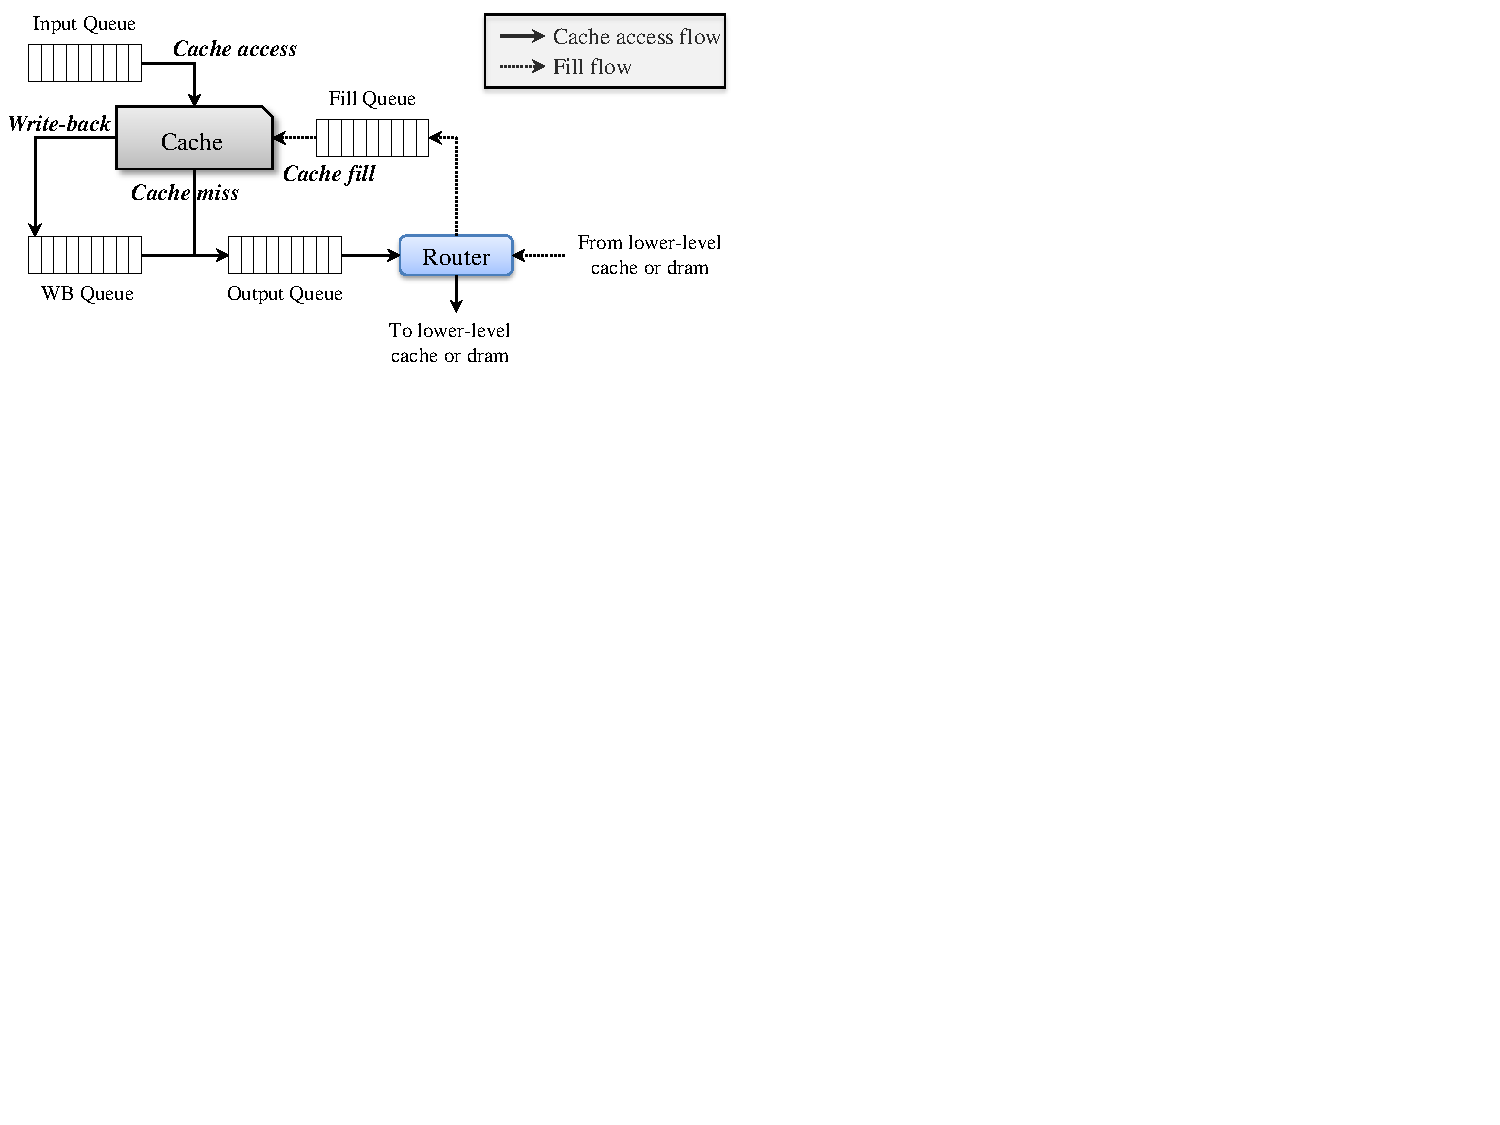
\includegraphics{figs/cache}
  \caption{The cache structure.}
  \label{fig:cache}
\end{figure*}

%%%%%%%%%%%%%%%%%%%%%%%%%%%%%%%%%%%%%%%%%%%%%%%%%%%%%%%%%%%%%%%%%%%%%%%%
\subsection{The Queues}
\label{sec:queue}
%%%%%%%%%%%%%%%%%%%%%%%%%%%%%%%%%%%%%%%%%%%%%%%%%%%%%%%%%%%%%%%%%%%%%%%%

\SIM uses queues to transfer data and command between different cache levels
and processors. Therefore, all cache accesses flow from one queue to another.
Below is the list of queues and their description.

\begin{itemize}
  \item \textbf{Input queue}: requests forwarded to the cache due to upper-level 
		cache misses or processor are inserted into this queue.

  \item \textbf{Output queue}: requests that miss in the cache are inserted into the
  output queue to be forwarded to a lower-level cache. If no lower-level cache
  is available, then requests are forwarded to the memory controller.

  \item \textbf{Write-back queue}: \SIM models write-back caches. When a dirty cache
  line is evicted, the line must be written back into the next level cache (or
  main memory). All write-back requests are initially inserted into this queue.

  \item \textbf{Fill queue}: Data returned from the next level cache or main memory 
  is inserted into the fill queue before updating the cache to be processed.

%  \item coherence queue - this queue is intended for handling coherence
%  traffic, but this is currently not modeled
  
\end{itemize}

%%%%%%%%%%%%%%%%%%%%%%%%%%%%%%%%%%%%%%%%%%%%%%%%%%%%%%%%%%%%%%%%%%%%%%%%
\subsection{The Flows}
\label{sec:cache-flow}
%%%%%%%%%%%%%%%%%%%%%%%%%%%%%%%%%%%%%%%%%%%%%%%%%%%%%%%%%%%%%%%%%%%%%%%%
In this subsection all possible flows from or to the cache is listed. If the memory or cache
levels are distributed, \SIM will use routers to send core's request. 

\begin{itemize}

  \item \textbf{Upper-level cache $\rightarrow$ Input queue}: Forwarding of upper-level cache misses
		to the cache.

  \item \textbf{Upper-level cache $\rightarrow$ Fill queue}: Forwarding of upper-level write-back 
		requests to the cache.

  \item \textbf{Input queue $\rightarrow$ Cache}: Accessing the cache

  \item \textbf{Cache $\rightarrow$ Output queue} : Cache miss, access to lower-level cache

  \item \textbf{Cache $\rightarrow$ Write-back queue}: Generating write-back requests due to
		eviction of a dirty line

  \item \textbf{Write-back queue $\rightarrow$ Output queue} : write-back requests to access the
		lower-level cache when they are processed.

  \item \textbf{Output queue $\rightarrow$ Router} : access the lower-level cache
		through the on-chip interconnection network

  \item \textbf{Router $\rightarrow$ Fill queue} : the data from the lower-level cache
		or DRAM

\end{itemize}

%%%%%%%%%%%%%%%%%%%%%%%%%%%%%%%%%%%%%%%%%%%%%%%%%%%%%%%%%%%%%%%%%%%%%%%%
\section{The Hierarchy}
\label{sec:memhierarchy}
%%%%%%%%%%%%%%%%%%%%%%%%%%%%%%%%%%%%%%%%%%%%%%%%%%%%%%%%%%%%%%%%%%%%%%%%

\SIM is very flexible in its support for different memory
hierarchies. Each level in the cache hierarchy can be configured
independently of other levels (see Section~\ref{sec:knob:cache}).
Figure~\ref{fig:memory} shows the base memory hierarchy without DRAM
memory. It is good to note these points about this figure: 

\begin{figure*}[htb]
\centering
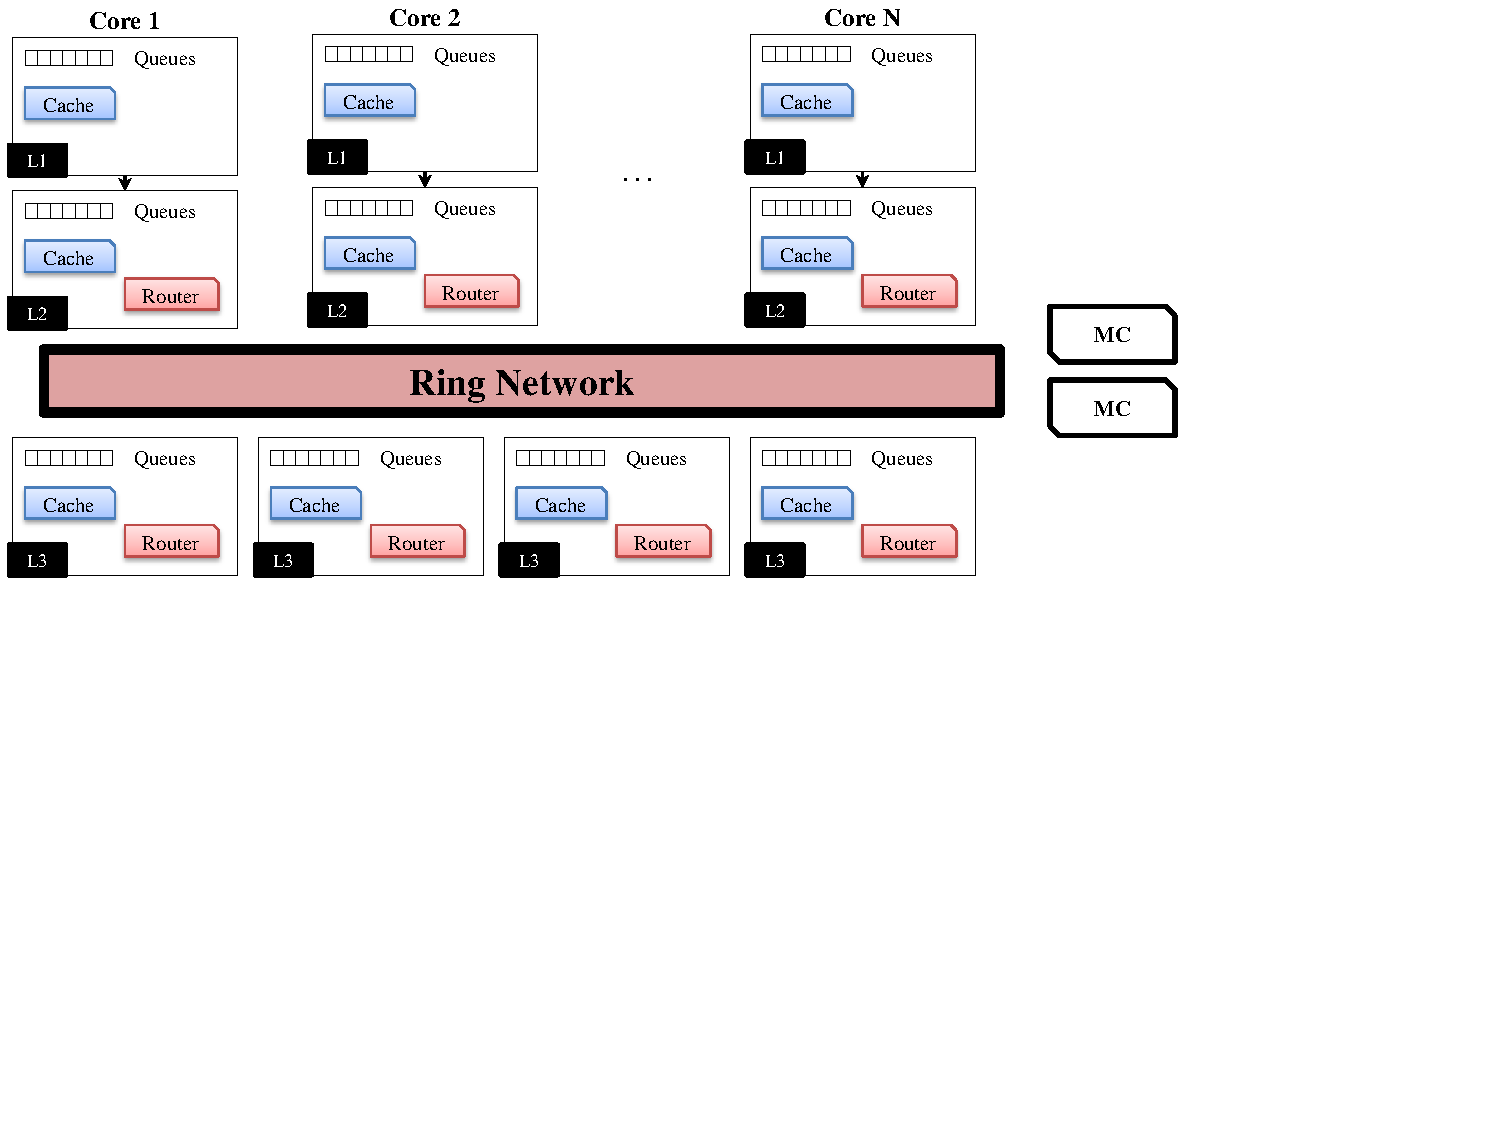
\includegraphics[width=6.5in]{figs/memory}
\caption{The memory system in \SIM.}
\label{fig:memory}
\end{figure*}


\begin{itemize} 
  \item There are three levels (L1, L2, and L3) of caches in the
	\SIM , the L2 cache can be disabled if needed.

  \item All the caches and memory controllers can be connected via an
    on-chip interconnection network (currently, the default topology
    is ring), if the configuration allows.

  \item L1 and L2 caches are always private to each core.

  \item The local router within a cache structure is enabled only when
	necessary.

  \item L3 cache is unified (shared by all cores), but sub banked. In
    other words, address regions are statically partitioned and each
    tile is responsible for sub regions. Each cache tile has multiple
    banks as well.
   
  \item Each L3 tile could be coupled with its own L2 to reduce network
	  traffic. This is controlled by knob \Verb+memory_type   l3_[de]coupled_network+.
	  For more setting for this knob look at \ref{sec:types_memory}.

\end{itemize}


Figure~\ref{fig:level2cache} shows how to configure a 2-level cache hierarchy.
Even though there are 3-levels of cache, the L2 cache is disabled and only its
router is used by the L1 cache to access the interconnection network. Since
there is no additional latency between L1 and L2 when the L2 is disabled, we
can flexibly configure 2-level cache hierarchies.


\begin{figure*}[htb]
\centering
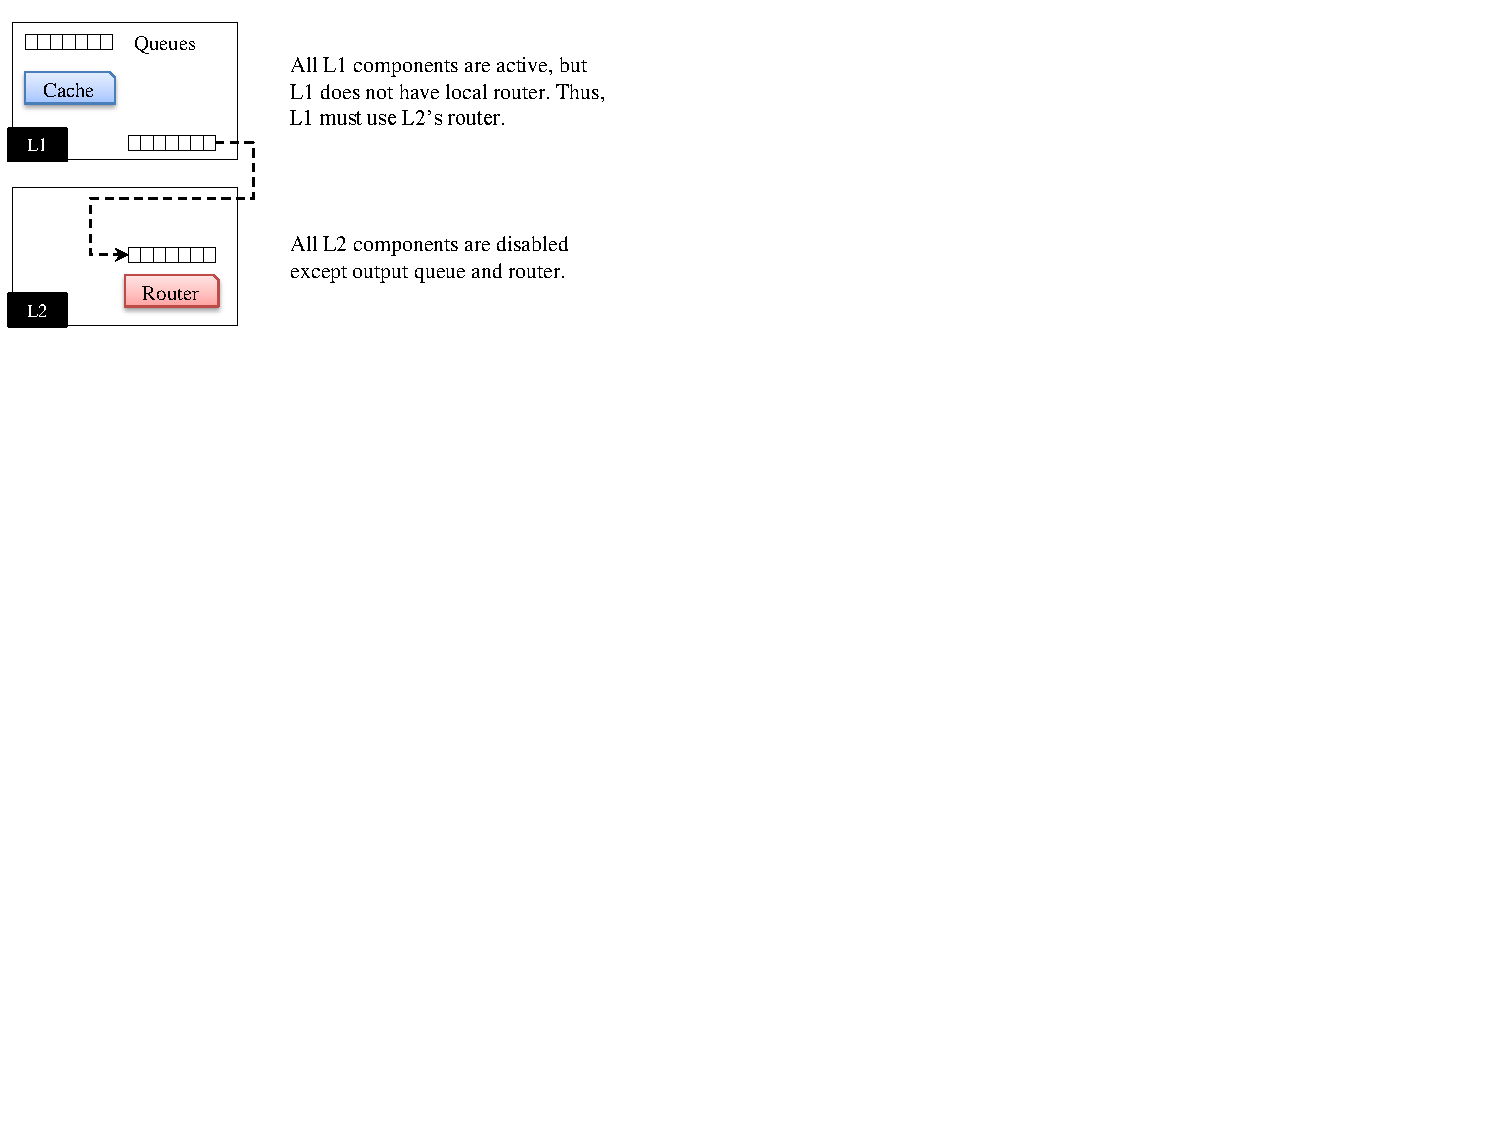
\includegraphics{figs/level2cache}
\caption{2-Level cache hierarchy.}
\label{fig:level2cache}
\end{figure*}

%%%%%%%%%%%%%%%%%%%%%%%%%%%%%%%%%%%%%%%%%%%%%%%%%%%%%%%%%%%%%%%%%%%%%%%%
\section{Configuring the Cache Hierarchy} 
%%%%%%%%%%%%%%%%%%%%%%%%%%%%%%%%%%%%%%%%%%%%%%%%%%%%%%%%%%%%%%%%%%%%%%%%

The cache hierarchy can be configured by:
\begin{enumerate}
 \item Setting the links between different cache levels
 \item Disabling cache levels
 \item Enabling/Disabling routers
\end{enumerate}
Following variables is used in \SIM for cache initialization:

\begin{center}
\begin{tabular}{l | l}
  Variable Name & Description \\ \hline \hline
  int next\_id & next level cache id \\
  int prev\_id & previous level cache id \\ 
  bool coupled\_up &  direct link with upper level cache \\
  bool coupled\_down & direct link with lower level cache \\
  bool disable & disable cache \\
  bool has\_router & router \\ 
\end{tabular}
\end{center}

\begin{description}
  \item[Enabling/disabling router] When \textsf{has\_router} is set to \textit{false},
  the cache cannot directly access to the on-chip
  interconnection. Instead, it has to go through lower-level cache's
  interface. Therefore, \textsf{coupled\_down} must set
  to \textit{true} and appropriate \textsf{next\_id} must be set. In
  this way, the output queue of the cache is connected directly to the
  input queue of the next level (lower) cache.

  \item[Disabling cache levels] When \textsf{disable} is set to \textit{true},
  the cache is disabled. When a request is inserted into the input queue of a
  disabled cache, the request will be directly inserted into the output queue
  of the cache. This feature has been used for modeling 2-level cache
  hierarchies. As Figure~\ref{fig:level2cache} shows, L1 and L3 caches are
  active, but L2 cache is disabled. However, since the L1 cache does not have a
  router, it needs to use the router of the L2 cache. Therefore,
  \textsf{has\_router} must be set to \textit{true} for the L2 cache.

  \item[Links] As mentioned in the Section~\ref{sec:memhierarchy}, the
  L1 and L2 caches are always private to a core. All L1 misses
  should go through the L2 cache without accessing the interconnection
  network. To this end, a direct link must be set between the L1 and
  L2 caches. Therefore, \textsf{coupled\_down} and \textsf{next\_id}
  must be set for the L1 cache and \textsf{coupled\_up}
  and \textsf{prev\_id} must be set for the L2 cache. Note that the
  link is always bi-directional.

\end{description}

%%%%%%%%%%%%%%%%%%%%%%%%%%%%%%%%%%%%%%%%%%%%%%%%%%%%%%%%%%%%%%%%%%%%%%%%
\subsection{Different Cache Hierarchies Configurations with \SIM}
\label{sec:types_memory}
%%%%%%%%%%%%%%%%%%%%%%%%%%%%%%%%%%%%%%%%%%%%%%%%%%%%%%%%%%%%%%%%%%%%%%%%
The configuration listed below could be used for knob \Verb+memory_type+.
In the description for each one the code for generating that configuration is
included.
\begin{itemize}
\ignore
		{
		\item Intel Core~\cite{core2duo} microarchitecture has two-level of
		caches. The last-level cache might be tiled, but if the L2 cache
		tries to access the closest the L3 tile, it does not have to access
		through the interconnection. All communications will be made through
		the direct link. However, if the L2 cache accesses the remote L3
		tile, it goes through the interconnection. Note that the number of
		cores (L1 and L2 caches) and the number of the L3 tiles must be the
		same.

		\smallskip
		\begin{lstlisting}
		// class l2_coupled_local_c
		\end{lstlisting}
		\smallskip
		 }

\item \textbf{l3\_coupled\_network}: Intel Nehalem~\cite{nehalem} and Sandy
    Bridge~\cite{sandybridge} microarchitectures have three-levels of
    caches. The last-level cache is tiled and to access the closest L3
    tile, a L2 cache does not have to go through the interconnection,
    it can access the L3 tile directly. However, if a L2 cache
    accesses a remote L3 tile, it goes through the interconnection.
    Note that the number of cores (L1 and L2 caches) and the number of
    the L3 tiles must be the same in this configuration.

\begin{Verbatim}
// class l3_coupled_network_c
for (int ii = 0; ii < m_num_core; ++ii) {
  // next_id, prev_id, done, coupled_up, coupled_down, disable, router
  m_l1_cache[ii]->init(ii, -1, false, false, TRUE, false, false);
  m_l2_cache[ii]->init(ii, ii, true,  TRUE,  TRUE, false, TRUE);
  m_l3_cache[ii]->init(-1, ii, false, TRUE,  false,false, TRUE);
}
\end{Verbatim}

  \item \textbf{no\_cache}: NVIDIA G80~\cite{g80} architecture does not have
  hardware-managed caches. Thus, all three levels are connected each
  other and disabled. Only the L3 cache has a router to access the DRAM.

  \begin{Verbatim}
  // class no_cache_c
  for (int ii = 0; ii < m_num_core; ++ii) {
    // next_id, prev_id, done, coupled_up, coupled_down, disable, router
    m_l1_cache[ii]->init(ii, -1, false, false, TRUE,  TRUE, false);
    m_l2_cache[ii]->init(ii, ii, true,  TRUE,  TRUE,  TRUE, false);
    m_l3_cache[ii]->init(-1, ii, false, TRUE,  false, TRUE, TRUE);
  }
  \end{Verbatim}

  \item \textbf{l2\_decoupled\_network}: NVIDIA Fermi~\cite{fermi} architecture has private L1 caches and a
  unified L2 cache shared by all cores. The L1 and L2 caches are linked. The L2
  cache is been disabled, but has its router enabled. The L3 is not linked with
  others (it is connected via the interconnect), but it is enabled and has a
  router.

  \begin{Verbatim}
  // class l2_decoupled_network_c
  // next_id, prev_id, done, coupled_up, coupled_down, disable, router
  for (int ii = 0; ii < m_num_core; ++ii) {
    m_l1_cache[ii]->init(ii, -1, false, false, TRUE,  false, false);
    m_l2_cache[ii]->init(-1, ii, true,  TRUE,  false, true,  true);
  }

  for (int ii = 0; ii < m_num_l3; ++ii) {
    // next_id, prev_id, done, coupled_up, coupled_down, disable, router
    m_l3_cache[ii]->init(-1, -1, false, false, false, false, true);
  }
  \end{Verbatim}
  
  \item \textbf{l3\_decoupled\_network} In a general 2-D Topology (Mesh, Torus), 
  it is assumed that each core has private L1 and L2 caches, but access to 
  the L3 cache must be through the interconnection network. The L1 and L2 caches 
  are both enabled and linked, but only the L2 cache has a router. The L3 cache is not linked
  with other caches and the communication is made through the interconnection
  network.

  \begin{Verbatim}
  // class l3_decoupled_network_c
  // next_id, prev_id, done, coupled_up, coupled_down, disable, router
  for (int ii = 0; ii < m_num_core; ++ii) {
    m_l1_cache[ii]->init(ii, -1, false, false, TRUE,  false, false);
    m_l2_cache[ii]->init(-1, ii, true,  TRUE,  false, false, TRUE);
  }

  for (int ii = 0; ii < m_num_l3; ++ii) {
    // next_id, prev_id, done, coupled_up, coupled_down, disable, router
    m_l3_cache[ii]->init(-1, -1, false, false, false, false, TRUE);
  }
  \end{Verbatim}
\end{itemize}


%%%%%%%%%%%%%%%%%%%%%%%%%%%%%%%%%%%%%%%%%%%%%%%%%%%%%%%%%%%%%%%%%%%%%%%%
\section{DRAM Module} 
\label{sec:dram}
%%%%%%%%%%%%%%%%%%%%%%%%%%%%%%%%%%%%%%%%%%%%%%%%%%%%%%%%%%%%%%%%%%%%%%%%

\SIM also models detailed memory controllers which consider DRAM
timing constraints and bandwidth specifications when scheduling
requests. Section~\ref{sec:param-dram} describes how to configure
DRAM parameters.

%%%%%%%%%%%%%%%%%%%%%%%%%%%%%%%%%%%%%%%%%%%%%%%%%%%%%%%%%%%%%%%%%%%%%%%%
\subsection{DRAM Timing Constraints}
%%%%%%%%%%%%%%%%%%%%%%%%%%%%%%%%%%%%%%%%%%%%%%%%%%%%%%%%%%%%%%%%%%%%%%%%

We model following three timing constraints of DRAM.

\vspace{0.2in}
\begin{center}
\begin{footnotesize}
\begin{tabular}{l l l l}
Timing              & Knob      				 & Symbol    & Description                         \\ \hline \hline
Precharge     		& \Verb+KNOB_DRAM_PRECHARGE+ & T$_{RP}$  & Row precharge time                  \\
Activate      		& \Verb+KNOB_DRAM_ACTIVATE+  & T$_{RCD}$ & Row address to column address delay \\
Column Access 		& \Verb+KNOB_DRAM_COLUMN+    & T$_{CL}$  & CAS latency                         \\
\end{tabular}
\end{footnotesize}
\end{center}

%%%%%%%%%%%%%%%%%%%%%%%%%%%%%%%%%%%%%%%%%%%%%%%%%%%%%%%%%%%%%%%%%%%%%%%%
\subsection{DRAM Bandwidth}
%%%%%%%%%%%%%%%%%%%%%%%%%%%%%%%%%%%%%%%%%%%%%%%%%%%%%%%%%%%%%%%%%%%%%%%%

DRAM bandwidth can be modeled using several factors:

\begin{center}
\vspace{0.2in}
\begin{footnotesize}
\begin{tabular}{l l}
Factor                                       & Knob 				     \\ \hline \hline
DRAM Frequency                      		 & \Verb+KNOB_DRAM_FREQUENCY+ \\
DRAM Data bus width                  	 	 & \Verb+KNOB_DRAM_BUS_WIDTH+  \\
Number of dram controllers            	 & \Verb+KNOB_DRAM_NUM_MC+    \\
Number of dram channels                  & \Verb+KNOB_DRAM_NUM_CHANNEL+    \\
\end{tabular}
\end{footnotesize}
\end{center}

\vspace{0.2in}
\noindent
Where $\textit{Bandwidth} = \textit{Frequency} \times \textit{Bus\_Width} \times 
	  \textit{Number\_of\_MemoryControllers} \times \textit{Number\_of\_Channels}$.
	  
%%%%%%%%%%%%%%%%%%%%%%%%%%%%%%%%%%%%%%%%%%%%%%%%%%%%%%%%%%%%%%%%%%%%%%%%
\subsection{The Structure of DRAM Controller}
%%%%%%%%%%%%%%%%%%%%%%%%%%%%%%%%%%%%%%%%%%%%%%%%%%%%%%%%%%%%%%%%%%%%%%%%

A DRAM controller consists of multiple banks and one or more channels.
Each bank has its own request buffer and request scheduler. The bank
scheduler picks a request to service based on the policy. Here are
some notes:

\begin{itemize}
  \item The bank scheduler picks a request based on the policy (FCFS,
    FR-FCFS, ...) if no request is being served currently.

  \item The channel scheduler picks a request from command-ready banks
    usually based on the policy (oldest-first). Based on the command,
    appropriate timing constraint (precharge, activate, or column
    access) is enforced to the bank.

  \item Once the column access signal is sent, the data is prepared
  from the DRAM chip (load) or the data is sent to the DRAM chip
  (store). Among multiple data-ready banks, the channel scheduler
  picks a request based on the policy (oldest-first).

  \item When the data is ready/sent for a request, the data is
  supplied to the cache (load) or the request is completed (store).

  \item If there are memory requests with the same address, these
  requests are merged into one dram request. 

\end{itemize}



% LocalWords:  prev bool microarchitecture Nehalem num init NVIDIA FCFS FRFCFS

%%%%%%%%%%%%%%%%%%%%%%%%%%%%%%%%%%%%%%%%%%%%%%%%%%%%%%%%%%%%%%%%%%%%%%%%
\chapter{Supporting {\gpu}s}
%%%%%%%%%%%%%%%%%%%%%%%%%%%%%%%%%%%%%%%%%%%%%%%%%%%%%%%%%%%%%%%%%%%%%%%%

MacSim can model {\gpu}s similar to NVIDIA's Tesla~\cite{lin:nic08} and
Fermi~\cite{fermi} architectures.  In these architectures the {\gpu} consists of a
scalable number of {\em Streaming Multiprocessors} (SMs), each containing
several {\em Scalar Processors} (SP) and {\em Special Function Units} (SFUs), a
multi-threaded instruction fetch and issue unit, a read-only constant cache, and
a read/write scratch pad memory called Shared Memory.  In \SIM, SMs are modeled
as cores and SPs as just one of the functional units. 


		\begin{figure}[htb]
		\centering
		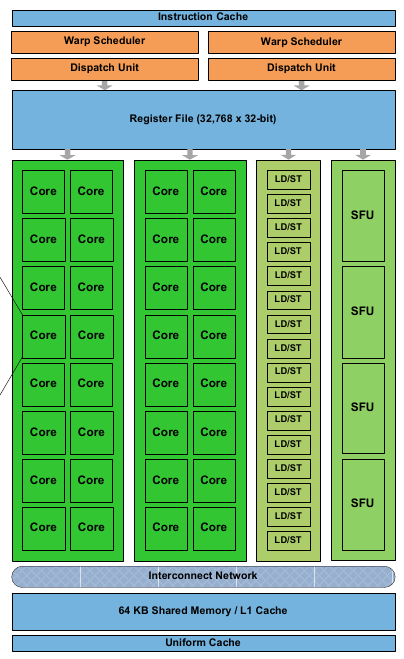
\includegraphics[scale=0.5]{figs/fermi_arch.png}
		\caption{An overview of the Fermi {\gpu} architecture}
		\label{fig:g80}
		\end{figure}

The behavior of certain components is different when simulating {\gpu}s, these
differences are described briefly below.

%%%%%%%%%%%%%%%%%%%%%%%%%%%%%%%%%%%%%%%%%%%%%%%%%%%%%%%%%%%%%%%%%%%%%%%%
\section{Traces}
\label{sec:ptx_traces}
%%%%%%%%%%%%%%%%%%%%%%%%%%%%%%%%%%%%%%%%%%%%%%%%%%%%%%%%%%%%%%%%%%%%%%%%

In NVIDIA {\gpu}s threads are executed in batches of 32 threads called
\textit{warps}. For simulating execution at warp granularity, for {\gpu}
applications, we generate traces at warp granularity. This means there
is one trace file per warp and each instruction in a trace file represents an
instruction executed by a warp. The instruction in the trace file encodes which
threads in the warp were active during the execution of the instruction. For
divergent branches, all instructions from one path are written to the trace
file first and only then instructions from the other path are written to the
trace file. For memory instructions, multiple instructions are written to the
trace file since each thread in a warp can access different addresses. Handling
of memory instructions inside the simulator is explained below.


%%%%%%%%%%%%%%%%%%%%%%%%%%%%%%%%%%%%%%%%%%%%%%%%%%%%%%%%%%%%%%%%%%%%%%%%
\section{Process Manager}
%%%%%%%%%%%%%%%%%%%%%%%%%%%%%%%%%%%%%%%%%%%%%%%%%%%%%%%%%%%%%%%%%%%%%%%%

The Process Manager (explained in Chapter~\ref{sec:process_manager})
does assignment of threads to cores (SMs) at block granularity - all
warps in the same thread block are assigned to the same core. The
number of blocks that can be assigned to each core is determined from
the resource requirement of each block and the {\gpu} architecture being
simulated.  This number is calculated at the time of trace generation
for compute devices of capability 2.0 and is included in the trace
files. This can also be specified by setting the knob
\Verb+max_block_per_core_super+.  For each block, the Process Manager
tracks the number of completed warps and when all warps in a block
have completed, the Process Manager retires the block and assigns a
new block to the core. The policy for assigning blocks to cores can be
different. Blocks could either be assigned statically to cores, or they
can be assigned to the first core that can accommodate the new block.

\ignore
		{\todo[inline]{support ..\_per\_core\_super per application}}

%%%%%%%%%%%%%%%%%%%%%%%%%%%%%%%%%%%%%%%%%%%%%%%%%%%%%%%%%%%%%%%%%%%%%%%%
\section{Memory Hierarchy}
%%%%%%%%%%%%%%%%%%%%%%%%%%%%%%%%%%%%%%%%%%%%%%%%%%%%%%%%%%%%%%%%%%%%%%%%

The following new components are added to the memory hierarchy for  - Shared Memory,
    Const Cache, Texture Cache.

%%%%%%%%%%%%%%%%%%%%%%%%%%%%%%%%%%%%%%%%%%%%%%%%%%%%%%%%%%%%%%%%%%%%%%%%
\section{Instruction Scheduler}
%%%%%%%%%%%%%%%%%%%%%%%%%%%%%%%%%%%%%%%%%%%%%%%%%%%%%%%%%%%%%%%%%%%%%%%%

A {\gpu}-specific (or a multithreaded architecture specific) instruction
scheduler is necessary, since neither single-threaded in-order nor
single-threaded out-of-order schedulers match the requirement of a {\gpu}
scheduler. A {\gpu} scheduler must be able to schedule instructions from
different warps while scheduling instructions from the same warp
in-order. A {\gpu}-specific scheduler is implemented in
\Verb+schedule_smc.cc+, this scheduler chooses instructions from
different warps. 

\ignore{\todo{round-robin order - not true!}}.

%%%%%%%%%%%%%%%%%%%%%%%%%%%%%%%%%%%%%%%%%%%%%%%%%%%%%%%%%%%%%%%%%%%%%%%%
\section{Simulating Memory Instructions}
%%%%%%%%%%%%%%%%%%%%%%%%%%%%%%%%%%%%%%%%%%%%%%%%%%%%%%%%%%%%%%%%%%%%%%%%

Due to the execution of threads at warp granularity, the execution of a memory
instruction generates multiple addresses, one from each thread. In the trace
file all the memory accesses are included as individual trace instructions, but
the accesses are marked as generated from the same memory instruction. During
simulation when it is detected that a sequence of memory accesses are from the
same memory instruction, the trace is read ahead until the end of the sequence
and the individual memory accesses are attached to a main uop as child uops. It
is the main uop that flows through the pipeline stages until execution. In the
execution stage it is detected that the main uop has several child uops and the
child uops that are issued to the memory hierarchy. When all the child uops
have completed, the main uop is ready for retirement.

\ignore
	  {
	  \missingfigure{better to add diagram from slide}
	  }

\ignore 
		{
		\subsection{Changes to support {\gpu}}
		\subsubsection{Front-end changes}
		The following components are modified to support {\gpu}s. 
		\begin{enumerate}
		\item Handling divergent branch
		\item Fetch scheduling (when to block a thread)
		\end{enumerate}
		\subsubsection{Scheduler}
		Different scheduling policy can be implemented. The default is the round-robin policy. 

		\subsubsection{Process Manager}

		\begin{enumerate}
		\item Block Dispatch: Threads are dispatched as a block granularity. 
		The simulator waits until all threads within a block are finished 
		before it dispatches another block. 
		\item Occupancy: When a trace is generated from Ocelot, it also emits the number of required 
		physical registers and memory usages. So the simulator uses that information to decide 
		how many blocks can be allocated for each core. This value can be overwritten by a KNOB as well. 
		\end{enumerate}

		\subsubsection{Execution Stage}
		Since one warp is treated as a functional unit, execution stage itself does not require too much change. Major changes are in handling uncoalesced memory  requests. 

		\subsubsection{Memory system}
		The simulator includes read-only cache, texture cache and constant cache to model {\gpu}s. 
		}

\ignore
		{
		Executing a warp instruction applies the instruction to 32 threads, similar to
		executing a SIMD instruction like an SSE instruction~\cite{sse} in X86.
		However, unlike SIMD instructions, the concept of warp is not exposed to the
		programmers, rather programmers write a program for one thread, and then
		specify the number of parallel threads in a block, and the number of blocks
		in a kernel grid. The Tesla architecture forms a warp using a batch of 32
		threads~\cite{cuda:course, sc2008_cuda} and in the rest of the paper we also
		use a warp as a batch of 32 threads.\ignore{\footnote{The CUDA
		manual~\cite{cuda_manual} describes a half warp (16 threads) as a minimum
		unit of execution. However, to simplify the model, we use only warp as a
		minimum unit of execution.}}

		All the threads in one block are executed on one SM together. One SM
		can also have multiple concurrently running blocks. The number of
		blocks that are running on one SM is determined by the resource
		requirements of each block such as the number of registers and shared
		memory usage. The blocks that are running on one SM at a given time
		are called {\em active blocks} in this paper. Since one block
		typically has several warps (the number of warps is the same as the
		number of threads in a block divided by 32), the total number of
		active warps per SM is equal to the number of warps per block times
		the number of active blocks.

		The shared memory is implemented within each SM multiprocessor as an
		SRAM and the global memory is part of the offchip DRAM. The shared
		memory has very low access latency (almost the same as that of
		register) and high bandwidth. However, since a warp of 32 threads
		access the shared memory together, when there is a bank conflict
		within a warp, accessing the shared memory takes multiple cycles.
		}


% LocalWords:  {\gpu} NVIDIA SMs SFUs multithreaded SPs {\gpu}s uncoalesced SIMD CUDA
% LocalWords:  SRAM offchip

%%%%%%%%%%%%%%%%%%%%%%%%%%%%%%%%%%%%%%%%%%%%%%%%%%%%%%%%%%%%%%%%%%%%%%%%
\chapter{\SIM Internals}
\label{sec:codetop}
%%%%%%%%%%%%%%%%%%%%%%%%%%%%%%%%%%%%%%%%%%%%%%%%%%%%%%%%%%%%%%%%%%%%%%%%

This chapter briefly discusses some internals of \SIM including data structures
and their purposes, important functions and components that will help users
understand \SIM better. For naming standards in \SIM code see chapter \ref{sec:add_macsim}.

%%%%%%%%%%%%%%%%%%%%%%%%%%%%%%%%%%%%%%%%%%%%%%%%%%%%%%%%%%%%%%%%%%%%%%%%
\section{run\_a\_cycle() function}
%%%%%%%%%%%%%%%%%%%%%%%%%%%%%%%%%%%%%%%%%%%%%%%%%%%%%%%%%%%%%%%%%%%%%%%%

All pipeline stages, units such as cache and memory controller, components such
as memory system and core implement their own \textit{run\_a\_cycle()} function which
is called every cycle. Within the \textit{run\_a\_cycle()} function of each
component the processing is done by the component for every simulation cycle.

\noindent \textit{macsim\_c}, the main simulation class, calls \textit{run\_a\_cycle()} for
the memory system, interconnect and cores in the simulation (see
\textit{macsim.cc}). Each core in turn calls \textit{run\_a\_cycle()} for
their own individual pipeline stages (see \textit{core.cc}).


%%%%%%%%%%%%%%%%%%%%%%%%%%%%%%%%%%%%%%%%%%%%%%%%%%%%%%%%%%%%%%%%%%%%%%%%
\section{Important data structures and classes}
%%%%%%%%%%%%%%%%%%%%%%%%%%%%%%%%%%%%%%%%%%%%%%%%%%%%%%%%%%%%%%%%%%%%%%%%

Here we list important data structures and classes in \SIM.

%%%%%%%%%%%%%%%%%%%%%%%%%%%%%%%%%%%%%%%%%%%%%%%%%%%%%%%%%%%%%%%%%%%%%%%%
\subsection{macsim\_c}
%%%%%%%%%%%%%%%%%%%%%%%%%%%%%%%%%%%%%%%%%%%%%%%%%%%%%%%%%%%%%%%%%%%%%%%%

For each simulation, an instance of \textit{macsim\_c} is created. This
instance is responsible for initializing the cores, the memory system, the
interconnection network and knobs, for registering classes/functions
implementing various policies with the factory classes and so on. Every cycle,
\textit{macsim\_c} ticks all the other simulation components via
the \textit{run\_a\_cycle()} function.

%%%%%%%%%%%%%%%%%%%%%%%%%%%%%%%%%%%%%%%%%%%%%%%%%%%%%%%%%%%%%%%%%%%%%%%%
\subsection{core\_c}
%%%%%%%%%%%%%%%%%%%%%%%%%%%%%%%%%%%%%%%%%%%%%%%%%%%%%%%%%%%%%%%%%%%%%%%%

Each core being simulated is represented by an object of \textit{core\_c}
declared in \textit{core.h}. Besides pointers to various pipeline stages and
hardware units, \textit{core\_c} tracks information such as how many threads
are assigned to the core, how many instructions have been fetched for each
thread and so on.

%%%%%%%%%%%%%%%%%%%%%%%%%%%%%%%%%%%%%%%%%%%%%%%%%%%%%%%%%%%%%%%%%%%%%%%%
\subsection{trace\_read\_c}
%%%%%%%%%%%%%%%%%%%%%%%%%%%%%%%%%%%%%%%%%%%%%%%%%%%%%%%%%%%%%%%%%%%%%%%%

An single instance of \textit{trace\_read\_c} is created at startup and is used
for reading the traces of all threads/warp in a simulation. To amortize the
overhead of reading traces, instructions are read from the trace file in chunks
instead of single instructions.

Some of the important functions in \textit{trace\_read\_c} are:

\begin{description}

  \item [get\_uops\_from\_traces()] called by front-end stage to fetch uops for a
	thread. If a decoded instruction is available, the next uop from the decoded
	instruction is returned to the front-end, otherwise the next instruction from
	the trace is decoded and the first uop from the decoded instruction is returned
	to the front-end.

  \item [read\_trace()] returns the next instruction from the trace buffer which
	contains a chunk of instructions read from the trace file. If the trace buffer
	is empty, a chunk is read from the trace file and the first instruction is
	returned.

  \item [convert\_pinuop\_to\_t\_uop()] decodes an instruction from a trace into a
	sequence of \textit{trace\_uop\_s} instances and returns the sequence.
	Instructions being decoded for the first time have their decoded information
	stored in a hashtable so that decoding does not have to be repeated when the
	same instruction is encountered again in the trace.

\end{description}

\ignore {\todo{add more if possible}}

%%%%%%%%%%%%%%%%%%%%%%%%%%%%%%%%%%%%%%%%%%%%%%%%%%%%%%%%%%%%%%%%%%%%%%%%
\subsection{map\_c}
%%%%%%%%%%%%%%%%%%%%%%%%%%%%%%%%%%%%%%%%%%%%%%%%%%%%%%%%%%%%%%%%%%%%%%%%

An instance of \textit{map\_c} is created for each core in the simulation. This
instance tracks data and memory dependences between the uops of a thread for all
threads assigned to a core. After a dependence is identified, the source uop is
added to a list of uops which should complete execution before the dependent
uop becomes ready for execution.

\ignore {\todo{add more if possible}}

%%%%%%%%%%%%%%%%%%%%%%%%%%%%%%%%%%%%%%%%%%%%%%%%%%%%%%%%%%%%%%%%%%%%%%%%
\subsection{uop\_c}
%%%%%%%%%%%%%%%%%%%%%%%%%%%%%%%%%%%%%%%%%%%%%%%%%%%%%%%%%%%%%%%%%%%%%%%%

An instance of \textit{uop\_c} defined in \textit{uop.h} is allocated (from a
pool) for each uop and is populated with all the information about the uop.
Each uop is assigned a unique number, \textit{m\_unique\_num}, that is unique
across all uops in a core. Each uop is also assigned a unique number,
\textit{m\_uop\_num}, that is unique across all uops of a thread. To
identify a uop from a thread of a core, \textit{m\_core\_id},
\textit{m\_thread\_id}, \textit{m\_uop\_num} member variables of the uop
have to checked. Users can define new member variables to collect/track
information as a uop moves through the pipeline. The \textit{uop\_c}
object allocated for a uop is returned to the \textit{uop\_c} pool when
the uop retires.  Whenever a new member variable is added to
\textit{uop\_c} users should make sure that the member variable is
initialized to a default value in \textit{uop\_c::init()}.

%%%%%%%%%%%%%%%%%%%%%%%%%%%%%%%%%%%%%%%%%%%%%%%%%%%%%%%%%%%%%%%%%%%%%%%%
\subsection{mem\_req\_s}
%%%%%%%%%%%%%%%%%%%%%%%%%%%%%%%%%%%%%%%%%%%%%%%%%%%%%%%%%%%%%%%%%%%%%%%%

For each memory request (L1 data cache miss, and write back requests), a
instance of \textit{mem\_req\_s} declared in \textit{memreq\_info.h} is
allocated. \textit{mem\_req\_s} contains all information relevant to a memory
request and an instance allocated to a request is freed only when the memory
request completes and data is filled in the cache. Users can define new member
variables to collect/track information as a memory request moves through the
memory hierarchy.

%%%%%%%%%%%%%%%%%%%%%%%%%%%%%%%%%%%%%%%%%%%%%%%%%%%%%%%%%%%%%%%%%%%%%%%%
\subsection{drb\_entry\_s}
%%%%%%%%%%%%%%%%%%%%%%%%%%%%%%%%%%%%%%%%%%%%%%%%%%%%%%%%%%%%%%%%%%%%%%%%

For each memory request that reaches the DRAM an instance of
\textit{drb\_entry\_s} declared in \textit{dram.h} is allocated. This instance
contains information about the bank, row and column of the DRAM request among
other details and is deallocated (freed) when the DRAM request is serviced.

%%%%%%%%%%%%%%%%%%%%%%%%%%%%%%%%%%%%%%%%%%%%%%%%%%%%%%%%%%%%%%%%%%%%%%%%
\subsection{rob\_c/smc\_rob\_c}
%%%%%%%%%%%%%%%%%%%%%%%%%%%%%%%%%%%%%%%%%%%%%%%%%%%%%%%%%%%%%%%%%%%%%%%%

\textit{rob\_c} declared in \textit{rob.h} and \textit{smc\_rob\_c} declared in
\textit{rob\_smc.h} are for ROBs in CPUs and GPUs respectively. uops are
allocated an entry in the ROB in the allocate stage and the allocated entry is
reclaimed when the uop retires.

%%%%%%%%%%%%%%%%%%%%%%%%%%%%%%%%%%%%%%%%%%%%%%%%%%%%%%%%%%%%%%%%%%%%%%%%
\subsection{pool\_c}
%%%%%%%%%%%%%%%%%%%%%%%%%%%%%%%%%%%%%%%%%%%%%%%%%%%%%%%%%%%%%%%%%%%%%%%%

\textit{pool\_c} defined \textit{utils.h} is a utility class meant for creating
memory pools. Using memory pools reduces the overhead of frequent memory
allocation and deallocation. In Macsim memory pools are used for uops
(\textit{uop\_c}), threads/warps (\textit{thread\_s}) and so on.

%%%%%%%%%%%%%%%%%%%%%%%%%%%%%%%%%%%%%%%%%%%%%%%%%%%%%%%%%%%%%%%%%%%%%%%%
\subsection{pqueue\_c}
%%%%%%%%%%%%%%%%%%%%%%%%%%%%%%%%%%%%%%%%%%%%%%%%%%%%%%%%%%%%%%%%%%%%%%%%

\textit{pqueue\_c} is a utility class for varying the length of the simulated
pipeline. In MacSim, it is used to vary the length of the fetch (and decode)
and allocation stages. At the time of creation of a \textit{pqueue\_c}
object, user has to specify the latency of the pqueue in cycles.
Objects/values enqueued into it are ready to be dequeued after specified
latency. Besides the object to be enqueued, the enqueue operation takes a
priority value as argument as well. Different priority values can be used for
objects enqueued in the same cycle to control which object gets dequeued
first from the pqueue.


%%%%%%%%%%%%%%%%%%%%%%%%%%%%%%%%%%%%%%%%%%%%%%%%%%%%%%%%%%%%%%%%%%%%%%%%
\section{Instructions Latencies}
%%%%%%%%%%%%%%%%%%%%%%%%%%%%%%%%%%%%%%%%%%%%%%%%%%%%%%%%%%%%%%%%%%%%%%%%

Latencies of X86 and PTX uops are defined in \textit{uoplatency\_x86.def} and
\textit{uoplatency\_ptx.def} files in \textit{def/}. Users must edit these
files to modify the latencies of instructions. Note that for PTX instructions,
the value defined in \textit{uoplatency\_ptx.def} is multiplied by the
value of the knob \textit{PTX\_EXEC\_RATIO}.


The process manager which is responsible for assigned threads (thread blocks)
to cores and data structures related to it are discussed in
Chapter~\ref{sec:process_manager}.

%%%%%%%%%%%%%%%%%%%%%%%%%%%%%%%%%%%%%%%%%%%%%%%%%%%%%%%%%%%%%%%%%%%%%%%%
\chapter{Process Manager/Thread Scheduler}
\label{sec:process_manager}
%%%%%%%%%%%%%%%%%%%%%%%%%%%%%%%%%%%%%%%%%%%%%%%%%%%%%%%%%%%%%%%%%%%%%%%%

MacSim uses a common Process Manager/Thread Scheduler for both CPU threads and
GPU warps. For each application that is to be simulated, the Process Manager
creates a process and also creates the threads/warps in the application. Based
on the simulation configuration, the Process Manager assigns cores to each
application, these cores are dedicated to the application. In case of CPU
applications, only the main thread of the application is launched first. The
trace configuration that is an input to the simulator specifies in terms of instructions
executed by the main thread when each child thread should be started. When a
child thread becomes ready for execution, the Process Manager is responsible
for assigning the child threads to cores. In case of GPU applications, the
Process Manager creates warps and forms thread blocks from these warps. The
thread blocks are assigned to cores according to the maximum number of blocks
supported by the core. Though the term core is commonly used for both x86 cores
and GPU cores, x86 threads can run only on a core
specified as x86 and a warp/block can run only a core specified as a GPU core.
Threads/warps once assigned to a core, remain attached to the core until they
terminate. When a thread or a warp terminates, the Process Manager is invoked
again for updating bookkeeping information. When it is determined that an
application can be terminated, based on the simulation parameters, the Process
Manager could repeat the simulation of the application until the termination
condition is met.

Some of the key data structures involved are:

\begin{description}

  \item [process\_s]: For each application that is to be simulated, the process manager
	creates a instance of type process\_s. This structure includes information such
	as process id, start information of threads, number of threads (warps) in
	the application, number of threads (warps) created, number of threads (warps)
	terminated, list of cores on which the application can run and so on.

  \item [thread\_s]: This structure is analogous to the task structure maintained by
	an operating system kernel. Each CPU thread and GPU warp has an instance of
	thread\_s structure. This structure includes fields for thread id (warp id),
	block id, pointer to trace file, process to which the thread belongs and
	other fields. 

  \item [block\_schedule\_info\_s]: Bookkeeping structure representing thread blocks in
	a GPGPU application. This structure contains fields for number of warps in a
	block, number of terminated warps, core to which the block is assigned and so
	on.

  \item [thread\_trace\_info\_node\_s]: Wrapper structure around thread\_s used by
	Process manager to track threads/warps yet to be assigned cores.

  \item [process\_manager\_c]: The class representing the process manager, an
	  instance of this class is created by the single instance of \textit{macsim\_c}
	  that is created for each simulation. Its operation is explained above, some of
	  the functions in \textit{process\_manager\_c} are:
	  
	  \begin{itemize}

		\item [create\_process()]: allocates \textit{process\_c} node for an
		  application. For CPU applications, \textit{create\_process()} reads the trace
		  configuration file and determines the number of threads in the application and their
		  start information. On the other hand, for GPU applications, it reads the trace
		  configuration file of the first kernel in the application and determines the number of
		warps and thread blocks in the kernel (calls \textit{setup\_process()} to do this).

		\item [terminate\_process()]: cleans up some data structures allocated for a
		  process and saves stats if it was the first run of a application. For GPU
		  applications, \textit{terminate\_process()}  terminates a kernel and calls
		  \textit{setup\_process()} which traces the trace configuration file for the next
		  kernel, determines the number warps and thread blocks in the kernel and calls
		  \textit{create\_thread\_node()}.

		\item [create\_thread\_node()]: is called for each thread/warp when it becomes
			ready for launch (note that all warps in a kernel are ready when the kernel is
			launched). \textit{create\_thread\_node()} allocates a
			\textit{thread\_trace\_info\_node\_s} node for a thread/warp and inserts the
			node into \textit{m\_thread\_queue} for threads and \textit{m\_block\_queue}
			for warps.

		\item [create\_thread()]: allocates an initializes a \textit{thread\_s} node, it
			also opens the trace file for the thread/warp for reading.


		\item [terminate\_thread()]: terminates a thread/warp, deallocates (returns to
			memory pool) data structures allocated for the thread/warp and calls
			\textit{sim\_thread\_schedule()}. For GPU applications,
			\textit{terminate\_thread()} retires a thread block if all warps in the block
			have completed. 


		\item [sim\_thread\_schedule()] assigns a thread to a core or a thread block to
		  a core if the number of threads/blocks assigned to the core are fewer than the
		  maximum allowed.

	  \end{itemize}

\end{description}


\begin{figure*}[htb]
\centering
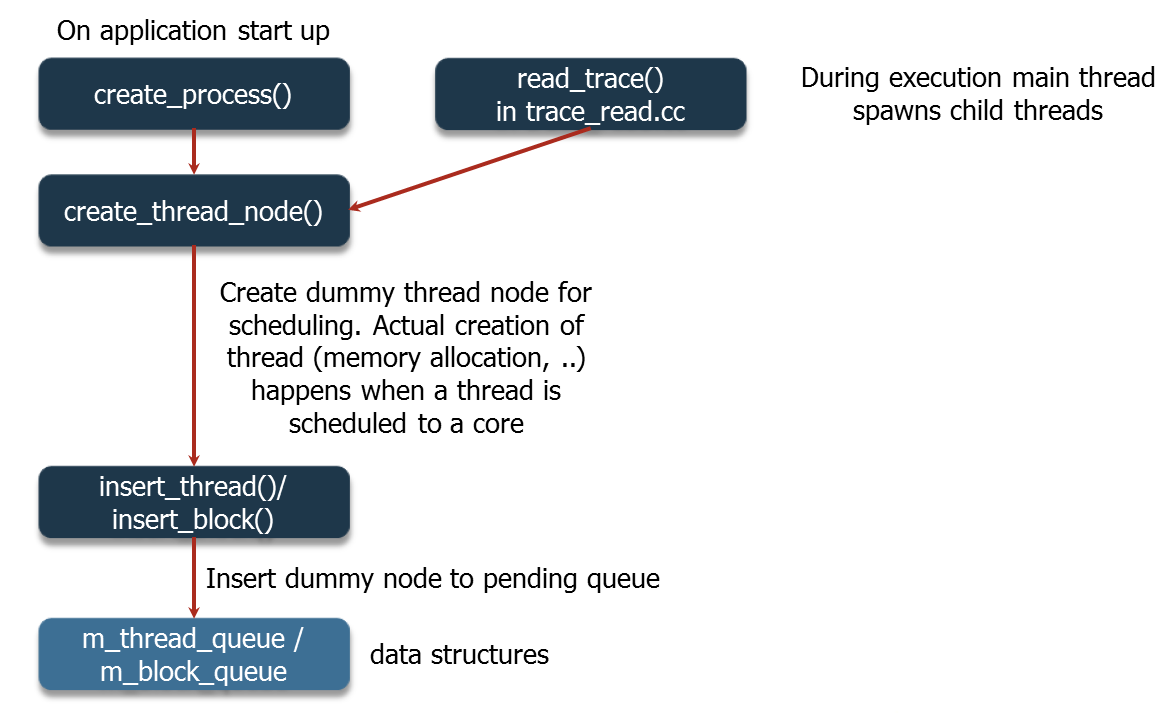
\includegraphics[height=80mm]{figs/process_creation}
\caption{Process and Thread Creation}
\label{fig:process_creation}
\end{figure*}

Figure~\ref{fig:process_creation} shows the control flow in the Process Manager on
simulation start up and during simulation. \textit{create\_process()} is called
for each application to be simulated. \textit{create\_process()} calls
\textit{setup\_process()} which in turn calls \textit{create\_thread\_node()}
for the main thread of the application. \textit{create\_thread\_node()}
allocates a \textit{thread\_trace\_info\_node\_s} instance for the main thread
and inserts it into \textit{m\_thread\_queue}. During the simulation of the
main thread when it is detected in \textit{read\_trace()} that a child thread
should be spawned, \textit{create\_thread\_node()} for the child thread is
called. The flow is similar for GPU kernels except that warps are inserted into
\textit{m\_block\_queue} instead of \textit{m\_thread\_queue}. Also, since GPU
kernels do not have a main thread, on kernel start up,
\textit{create\_thread\_node()} is called for the first warp in the
kernel. 

\begin{figure*}[htb]
\centering
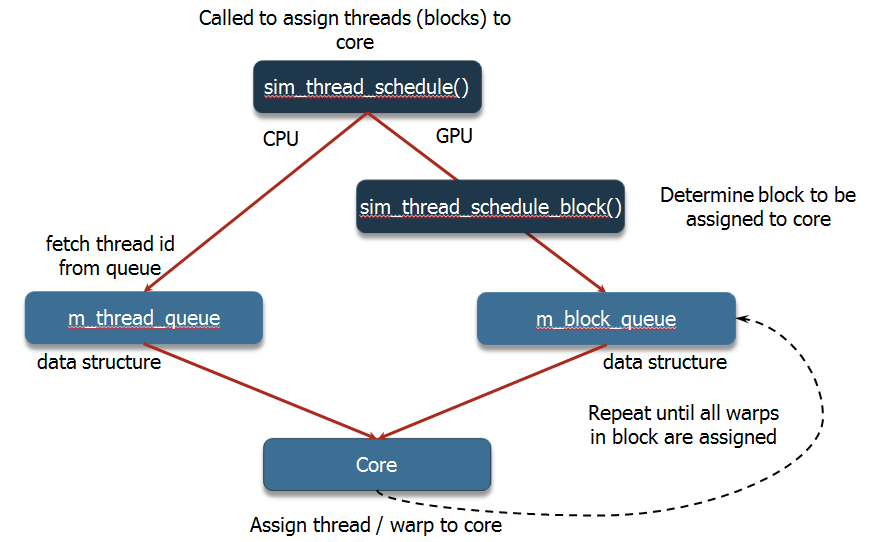
\includegraphics[height=80mm]{figs/thread_scheduling}
\caption{Thread/Thread Block Scheduling}
\label{fig:thread_scheduling}
\end{figure*}

When a thread/warp running on a core terminates,
\textit{sim\_thread\_schedule()} is called to schedule new threads/thread
blocks onto the core. Note that a new thread block can be assigned to a
core only when all warps of a previously assigned block have terminated.
\textit{sim\_thread\_schedule()} removes threads/warps from
\textit{m\_thread\_queue/m\_block\_queue} and assigns them to the core.
This flow is shown in Figure~\ref{fig:thread_scheduling}.


%%%%%%%%%%%%%%%%%%%%%%%%%%%%%%%%%%%%%%%%%%%%%%%%%%%%%%%%%%%%%%%%%%%%%%%%
\chapter{Adding to \SIM}
\label{sec:add_macsim}
%%%%%%%%%%%%%%%%%%%%%%%%%%%%%%%%%%%%%%%%%%%%%%%%%%%%%%%%%%%%%%%%%%%%%%%%
In this chapter procedure to add new policies, predictors and prefetcher 
to \SIM are explained.

%%%%%%%%%%%%%%%%%%%%%%%%%%%%%%%%%%%%%%%%%%%%%%%%%%%%%%%%%%%%%%%%%%%%%%%%
\section{New DRAM Policy}
%%%%%%%%%%%%%%%%%%%%%%%%%%%%%%%%%%%%%%%%%%%%%%%%%%%%%%%%%%%%%%%%%%%%%%%%


To implement a new DRAM scheduling policy, a class that extends
\textit{dram\_controller\_c} has to be defined. This class should
overload the \textit{schedule()} function which should return the next
DRAM request to be serviced according to the policy. Please refer to
class \textit{dc\_frfcfs\_s} defined in dram.cc/h for a sample. In
addition to the class, define a wrapper function that returns an
instance of the class (see \textit{dram.cc} for an example) and
register the class with the DRAM factory (see \textit{see
register\_functions() in \textit{macsim.cc}}.


%%%%%%%%%%%%%%%%%%%%%%%%%%%%%%%%%%%%%%%%%%%%%%%%%%%%%%%%%%%%%%%%%%%%%%%%
\section{New Instruction Scheduler}
%%%%%%%%%%%%%%%%%%%%%%%%%%%%%%%%%%%%%%%%%%%%%%%%%%%%%%%%%%%%%%%%%%%%%%%%

Define a class that extends \textit{schedule\_c} and overloads at least the
\textit{run\_a\_cycle()} function. Other functions may be overloaded to
maintain a consistent code structure across the different instruction
schedulers. After defining the new scheduler, add code to \textit{core.cc} to
instantiate the new scheduler instead of one of the provided schedulers.

%%%%%%%%%%%%%%%%%%%%%%%%%%%%%%%%%%%%%%%%%%%%%%%%%%%%%%%%%%%%%%%%%%%%%%%%
\section{New policy for assigning thread blocks to GPU cores}
%%%%%%%%%%%%%%%%%%%%%%%%%%%%%%%%%%%%%%%%%%%%%%%%%%%%%%%%%%%%%%%%%%%%%%%%

In \textit{process\_manager\_c::sim\_schedule\_thread\_block()} add (or modify)
code to determine the id of the block that will be assigned to the core based
on the new policy. The list of ready blocks can be obtained via
\textit{m\_block\_schedule\_info} member of the \textit{macsim\_c} object that
is created for the simulation.

%%%%%%%%%%%%%%%%%%%%%%%%%%%%%%%%%%%%%%%%%%%%%%%%%%%%%%%%%%%%%%%%%%%%%%%%
\section{New Fetch Policy}
\label{sec:modify:fetch}
%%%%%%%%%%%%%%%%%%%%%%%%%%%%%%%%%%%%%%%%%%%%%%%%%%%%%%%%%%%%%%%%%%%%%%%

There are several steps to add a new thread fetching policy. We will
provide an example with round-robin fetch policy, which is already
provided by \SIM.

\begin{enumerate}[Step 1.]
\item Define a new fetch policy in \Verb+class frontend_c+.
\begin{Verbatim}
// frontend.h
class frontend_c {
  ...
  int fetch_rr(void);
  ...
}
\end{Verbatim}

\item Implement this new policy.

\item Register this new policy in \Verb+macsim.cc+.
\begin{Verbatim}
fetch_factory_c::get()->register_class("rr", fetch_factory);
\end{Verbatim}


\item Assign this policy to \Verb+MT_fetch_Scheduler+ in \Verb+frontend.cc+.
\begin{Verbatim}
if (policy == ``rr'') {
  MT_fetch_scheduler = &frontend_c::fetch_rr;
}
\end{Verbatim}

\item Enable this new branch predictor by setting \Verb+KNOB_FETCH_POLICY+.
\begin{Verbatim}
./macsim --fetch_policy=rr     -- in the commandline
fetch_policy rr                -- in the params.in
\end{Verbatim}
\end{enumerate}


%%%%%%%%%%%%%%%%%%%%%%%%%%%%%%%%%%%%%%%%%%%%%%%%%%%%%%%%%%%%%%%%%%%%%%%%
\section{New Branch Predictor}
%%%%%%%%%%%%%%%%%%%%%%%%%%%%%%%%%%%%%%%%%%%%%%%%%%%%%%%%%%%%%%%%%%%%%%%%

There are several steps to add a new branch predictor. We will provide
an example with gshare~\cite{mcf93} branch predictor, which is already
provided by \SIM.

\begin{enumerate}[Step 1.]
  \item Define a new class which inherits \Verb+class bp_dir_base_c+
\begin{Verbatim}
class bp_gshare_c : public bp_dir_base_c {};
\end{Verbatim}

  \item Define and implement other necessary features of a new branch
    predictor. Especially, override \Verb+pred()+, \Verb+update()+,
    and \Verb+recover()+ functions.
\begin{Verbatim}
uns8 bp_gshare_c::pred(uop_c* uop) {...}
void bp_gshare_c::update(uop_c* uop) {...}

\end{Verbatim}

  \item Add a policy to the branch predictor factory in
    \Verb+macsim.cc+ and to the allocator in \Verb+bp.cc+.

\begin{Verbatim}
// macsim.cc macsim_c::register_functions()
bp_factory_c::get()->register_class(``gshare'', default_bp);

// bp.cc
bp_dir_base_c* default_bp(macsim_c* simBase)
{
  ...
  else if (bp_type == ''gshare'')
    new_bp = new bp_gshare_c(simBase);
  ...
}
\end{Verbatim}

  \item Enable this new branch predictor by setting \Verb+KNOB_BP_DIR_MECH+.
\begin{Verbatim}
./macsim --bp_dir_mech=gshare     -- in the commandline
bp_dir_mech gshare                -- in the params.in
\end{Verbatim}
\end{enumerate}


%%%%%%%%%%%%%%%%%%%%%%%%%%%%%%%%%%%%%%%%%%%%%%%%%%%%%%%%%%%%%%%%%%%%%%%%
\section{New Hardware Prefetcher}
%%%%%%%%%%%%%%%%%%%%%%%%%%%%%%%%%%%%%%%%%%%%%%%%%%%%%%%%%%%%%%%%%%%%%%%%

There are several steps to add a new hardware prefetcher. We will provide
an example with a stride~\cite{iac:spr04} prefetcher, which is already
provided by \SIM.

\begin{enumerate}[Step 1.]
  \item Define a new class which inherits \Verb+class pref_base_c+
\begin{Verbatim}
class pref_stride_c : public pref_base_c {};
\end{Verbatim}

  \item Define and implement other necessary features of a new
    hardware prefetcher. Especially, override several function.
\begin{Verbatim}
void init_func(int);                            // on initiation of prefetch request
void done_func();                               // when a prefetch request is installed
void l1_miss_func(int, Addr, Addr, uop_c*);     // on L1 miss
void l1_hit_func(int, Addr, Addr, uop_c*);      // on L1 hit
void l1_pref_hit_func(int, Addr, Addr, uop_c*); // on L1 prefetch hit
void l2_miss_func(int, Addr, Addr, uop_c*);     // on L2 miss
void l2_hit_func(int, Addr, Addr, uop_c*);      // on L2 hit
void l2_pref_hit_func(nt, Addr, Addr, uop_c*);  // on L2 prefetch hit
\end{Verbatim}

  \item Add a prefetcher to the prefetcher factory in \Verb+pref_factory.cc+.

\begin{Verbatim}
// pref_factory.cc
void pref_factory(...)
{
  pref_base_c* pref_stride = new pref_stride_c(...);
  pref_table.push_back(pref_stride);
  ...
}
\end{Verbatim}

  \item Enable this new hardware prefetcher by setting
    \Verb+KNOB_PREF_STRIDE_ON+ (please refer to pref\_stride.cc
    pref\_stride\_c::pref\_stride\_c()). \textit{Note that the way we
      simulate hardware prefetchers are not same as other modules.}
\begin{Verbatim}
switch (type) {
  case UNIT_SMALL:
    knob_enable = *m_simBase->m_knobs->KNOB_PREF_STRIDE_ON;
      break;
    case UNIT_MEDIUM:
      knob_enable = *m_simBase->m_knobs->KNOB_PREF_STRIDE_ON_MEDIUM_CORE;
      break;
    case UNIT_LARGE:
      knob_enable = *m_simBase->m_knobs->KNOB_PREF_STRIDE_ON_LARGE_CORE;
      break;
}

./macsim --pref_stride_on[,medium_core, large_core]=1
pref_stride_on[,medium_core, large_core] 1
\end{Verbatim}
\end{enumerate}

%%%%%%%%%%%%%%%%%%%%%%%%%%%%%%%%%%%%%%%%%%%%%%%%%%%%%%%%%%%%%%%%%%%%%%%%
\chapter{Troubleshooting Information}
\label{sec:troubleshooting}
%%%%%%%%%%%%%%%%%%%%%%%%%%%%%%%%%%%%%%%%%%%%%%%%%%%%%%%%%%%%%%%%%%%%%%%%
This chapter contains information that might be useful when you encounter 
a problem in building, running \SIM.

%%%%%%%%%%%%%%%%%%%%%%%%%%%%%%%%%%%%%%%%%%%%%%%%%%%%%%%%%%%%%%%%%%%%%%%%
\section{Error opening trace file}
%%%%%%%%%%%%%%%%%%%%%%%%%%%%%%%%%%%%%%%%%%%%%%%%%%%%%%%%%%%%%%%%%%%%%%%%

If you encounter ``error opening trace file \ldots'' error message when you run \SIM, it is highly likely because of your operating system's restriction on the maximum number of open file descriptors. At the time of writing, by default, Mac OS X (10.10.5 Yosemite) sets the maximum number of open file descriptor, 256; whereas it is 1024 in Ubuntu 14.04. Once the number of maximum files is reached, trace cannot be opened and the simulation aborts. If this is the case, then simply increase the limitation with ``ulimit -n <N>'' command.

%%%%%%%%%%%%%%%%%%%%%%%%%%%%%%%%%%%%%%%%%%%%%%%%%%%%%%%%%%%%%%%%%%%%%%%%%
\chapter{Debugging}
\label{sec:debugging}
%%%%%%%%%%%%%%%%%%%%%%%%%%%%%%%%%%%%%%%%%%%%%%%%%%%%%%%%%%%%%%%%%%%%%%%%

TBD 

%%%%%%%%%%%%%%%%%%%%%%%%%%%%%%%%%%%%%%%%%%%%%%%%%%%%%%%%%%%%%%%%%%%%%%%%
\section{Forward Progress Error}
%%%%%%%%%%%%%%%%%%%%%%%%%%%%%%%%%%%%%%%%%%%%%%%%%%%%%%%%%%%%%%%%%%%%%%%%


%%%%%%%%%%%%%%%%%%%%%%%%%%%%%%%%%%%%%%%%%%%%%%%%%%%%%%%%%%%%%%%%%%%%%%%%
\section{Debugging with Debugging Messages}
%%%%%%%%%%%%%%%%%%%%%%%%%%%%%%%%%%%%%%%%%%%%%%%%%%%%%%%%%%%%%%%%%%%%%%%%

To check the correctness of the module, We provide debugging features
with text-based debugging messages. For example,

\begin{Verbatim}
debug message example
\end{Verbatim}

You can define anywhere. Opt version will nullify these statement for
performance purpose.

enable variable

To enable debug messages \Verb+make dbg+ and 

\begin{Verbatim}
debug_cycle_start
debug_cycle_end
\end{Verbatim}

debug macros are defined in \Verb+src/debug_macros.h+

debug macro is very similar to \Verb+printf+ function.

\begin{Verbatim}
_debug(debug_variable, const char * format, ... )
\end{Verbatim}

\begin{Verbatim}
#define DEBUG(args...) _DEBUG(*m_simBase->m_knobs->KNOB_DEBUG_MEM, ## args)
\end{Verbatim}


useful data for 

\begin{Verbatim}
core id
thread id
uop num
inst num
vaddr
req_id
\end{Verbatim}


To add a new debug stage, you need to add a debug knob variable in debug.param.def


%\begin{Verbatim}
%DEBUG(
%\end{Verbatim}

%the meanting of debug statements. 
%How to turn on debug flags for different modules

%\subsection{DE


%\subsection{Debug Knob Variables}

%All debug variabls are defined in \Verb+macsim-top/trunk/def/debug.param.def+



%how to enable

%debug_start_cycle debug_end_cycle

%grep core_id thread_id

%how to add a new stage


%\subsection{How to Add Debugging Messages}

%\begin{enumerate}
%\item Add a new debug variable
%\item Add debug macro in files
%\item DEBUG
 %Still incomplete
%
\chapter{Internal Users Only Manual}
\section{Regression Tests}
\label{sec:regression}

To confirm your change does not affect the behavior of other parts,
regression test can be an useful tool. Let's say your current working
directory name is macsim-working. Here are steps to perform regression
test.

\begin{enumerate}[Step 1.]

\item You need to get a clean copy of macsim again. Let's say you are
  getting a new copy in macsim-regression directory.

\begin{Verbatim}
svn co https://svn.research.cc.gatech.edu/macsim/trunk macsim-regression --username user
\end{Verbatim}

\item You have to get a simulator tool, which is in the hparch svn
  repository.

\begin{Verbatim}
svn co https://svn.research.cc.gatech.edu/hparch/sim/trunk/tools tools --username user
\end{Verbatim}

\item Go to macsim-regression/trunk/bin directory and execute
  \Verb+regression_gen.py+ which is in your tool directory.

\begin{Verbatim}
cd macsim-regression/bin
regression_gen.py
\end{Verbatim}

\item Go to macsim-working/bin directory and execute
  \Verb+regression_test.py+ which is in your tool directory.

\begin{Verbatim}
cd macsim-working/bin
regression_test.py
\end{Verbatim}

\item Here is the output.

\begin{Verbatim}
regression_test.py
running ptx_fermi_6core BicubicTexture - 1 of 123
running ptx_fermi_6core BlackScholes1 - 2 of 123
running ptx_fermi_6core ConvolutionSeparable - 3 of 123
running ptx_fermi_6core ConvolutionTexture - 4 of 123
running ptx_fermi_6core Dct8x8 - 5 of 123
running ptx_fermi_6core Dxtc1 - 6 of 123
running ptx_fermi_6core FastWalshTransform - 7 of 123
running ptx_fermi_6core Histogram2561 - 8 of 123
...
Summary: total 123 pass 123 diff 0 fail 0
\end{Verbatim}

\end{enumerate}


\section{What to use internal directory}

TBD

 %For internal users only
%

\chapter{FAQ}
\label{sec:faq}

This chapter answers some frequently asked questions.

\begin{enumerate}[Q 1.]
  \item I'd like to add a new file in Macsim. What should I do? 

\begin{enumerate}[1.]
\item First add files in src directory.
\item Add an entry in macsim/trunk/.obj/Makefile.am.
\begin{Verbatim}
  all_sources = \
    ... \
    ../src/new_file.cc
\end{Verbatim}
\end{enumerate}

\end{enumerate}
 %Still incomplete
%
\clearpage
\section{Tools}
\label{sec:tool}
TBD 
\subsection{Trace Reader}
TBD 
 %Empty, For tools folder
%
\clearpage
\section*{Acknowledgments}

Acknowledgments...



 %Empty, Acknoledgements

\bibliographystyle{ieee}
\bibliography{ref}


%\begin{thebibliography}{9}
%\bibliography{ref}
%\end{thebibliography}



\clearpage
\appendix

\chapter{Coding Style Guideline}


\section{Naming Conventions}

Names should be as descriptive as possible, do not hesitate to use
long names.  Shorten names only when the purpose of the name can still
be understood clearly.


\subsection{Classes}

\begin{itemize}

  \item \textbf{Class names} should use lower case alphabets only.  If the name
consists of multiple words, then the words should be separated using
the underscore character. Class names should end with c.  Eg.

\begin{Verbatim}
class  my_class_c;
\end{Verbatim}


  \item \textbf{Class member variables} should use the prefix m .  Member variable
names should use lower case alphabets only, multiple words should be
separated using the underscore character.  Eg.

\begin{Verbatim}
int  m_instance_variable;
\end{Verbatim}


  \item \textbf{Accessor i.e, get/set, member functions} should use
the names of the corresponding member variables without the m
suffix. In addition, the set functions should use the prefix set ,
while no prefix is needed for the get functions.  Eg.


\begin{Verbatim}
int  m_my_variable;
...
...
void  set_my_variable(int);
int  my_variable();
\end{Verbatim}


  \item \textbf{Other member functions} should always start with a
verb, multiple words should be separated with the underscore character
and no upper case letters are allowed.  Eg.

\begin{Verbatim}
int  access_cache();
\end{Verbatim}


  \item Example class declaration

\begin{Verbatim}
class  my_class_c  {
  private:
    int  m_var_one;
    bool  m_var_two;
    ...
    ...

    void  set_var_one(int);
    int  var_one();
    ...
    int  check_values();
};
\end{Verbatim}

\end{itemize}





\subsection{Structures}

\begin{itemize}

  \item Structure names should use lower case alphabets only. If the
name consists of multiple words, then the words should be separated
using the underscore character. Structure names should end with s. Eg.

\begin{Verbatim}
struct  my_struct_s;
\end{Verbatim}

  \item Do not use any prefix or suffix for structure member
  variables.

  \item Example structure declaration

\begin{Verbatim}
typedef struct my_type_s  {
  type field_one;
  type field_two;
}  my_type_s;
\end{Verbatim}

\end{itemize}





\subsection{Other Types}

Other user defined types should use only lower case letters with
multiple words being separated by the underscore character. These
types should use the suffix t.  Eg.

\begin{Verbatim}
typedef  std::map<int,  std::list<int>  > my_type_t;
\end{Verbatim}


\subsection{Global Variables}

Global variable names should use the prefix g and use lower case
letters only, multiple words should be separated by the underscore
character.  Eg.

\begin{Verbatim}
int  g_my_global_variable;
\end{Verbatim}


\subsection{Local Variables}

Local variables follow the same convention as global variables, except
that they do not require the g prefix.  Eg.

\begin{Verbatim}
int  my_local_variable;
\end{Verbatim}


\subsection{Constant  Variables}

Constant variables follow the same convention as global variables,
except that they use the prefix k , instead of g .  Eg.

\begin{Verbatim}
const  int  k_my_const  = 25;
\end{Verbatim}


\subsection{Macros}

Macro names should use upper case letters only with multiple words
being separated my underscores. Eg.

\begin{Verbatim}
#define  MAX_NUM_THREADS  8192
\end{Verbatim}




\section{Formatting and Readability}

\subsection{Indentation}

Use only spaces for indentation, do not use tabs.  The indentation
must be two spaces wide.


\subsection{Variable Declaration}

Variables should be declared at the point in the code where they are
needed, and should be assigned an initial value at the time of
declaration.


\subsection{Control Statements and Function Definitions}

\begin{itemize}

  \item For \textit{if}, \textit{for}, \textit{while}
and \textit{switch} statements, there should be a single single space
between the keyword and the opening parenthesis.  The opening curly
brace should appear on the same line as the statement and there should
be a single space between the closing parenthesis and the opening
curly brace.  The opening curly brace following a do statement must
also follow the same rules.  The \textit{while} of a \textit{do while}
loop should be on the same line as the closing parenthesis of the loop
body and should be separated from the closing parenthesis by a single
space.  Eg.

\begin{Verbatim}
//correct
if (condition)  { 
  statement 1; 
  statement 2;
}

//correct
for  (int  ii = 0;  ii < N;  ++ii)  {
  statement 1;
  statement 2;
}

//correct
while  (condition)  { 
  statement 1; 
  statement 2;
}

//correct
switch  (variable)  {
  condition 1: 
    statement 1; 
    break;
  condition 2: 
    statement 2; 
    break;
  default: 
    statement 3; 
    break;
}

//correct 
do {
  statement 1;
  statement 2;
} while (condition);
\end{Verbatim}



  \item \textit{else} statements should be on the line following the
closing parenthesis of the corresponding if block. There should be a
single space between the else keyword and the opening curly brace of
the else block. The same rules apply for \textit{else if} statements
as well.  Eg.

\begin{Verbatim}
//correct
if (test_cond)  {
...
}
else  {
...

}

//correct
if (test_cond)  {
...
}
else  if (another_cond)  {
...
}
\end{Verbatim}

  \item When defining functions, there should be no spaces between the
function name and the opening parenthesis, there should be a single
space between the closing parenthesis and the opening curly brace which
should appear on the same line as the function name.  Eg.

\begin{Verbatim}
//correct
int  my_func_defn(int  arg_a,  int  arg_b)  {
  ...
}
\end{Verbatim}
\end{itemize}


\subsection{Horizontal Spacing}

Except for when using the operators listed below use a single space
between the operator and the operands (note the slight difference in
using the comma operator).  For the operands listed below, spaces
should not be used.  List of operators which do not need horizontal
spacing:

\begin{Verbatim}
() [] ->    ++ -- + - ! ~  (type)  *  &   sizeof
\end{Verbatim}

Eg.

\begin{Verbatim}
i = j + k * i;     // correct 
i = j+k*i;         // wrong

array[i]  = j;     // correct 
array [i] = j;     // wrong

my_func(a, b, c);  // correct 
my_func(a,b,c);    // wrong
\end{Verbatim}



\subsection{Statements}

Each statement should be on its own line, this applies to variable
declarations as well. Eg.

\begin{Verbatim}
int i = 0;          // correct 
int j = 0;          // correct
int i = 0,  j = 0;  // wrong 
i++;                // correct
j++;                // correct

i++;  j++;          // wrong 
i = 0;  j = 0;      // Wrong
\end{Verbatim}



\subsection{Column Length}

Lines should not exceed more than 80 characters in length.  If a line
is longer than 80 characters, split it into multiple lines.


\section{Header Files and Include Directives}

\begin{itemize}

  \item All header files should have an ``include guard'' to prevent
  accidental inclusion of the file multiple times in a single
  compilation unit.  The include guard should be named after the file
  name.  Eg.

\begin{Verbatim}
// in  pref_common.h
#ifndef  PREF_COMMON_H  #define  PREF_COMMON_H
...
...
#endif
\end{Verbatim}


  \item Avoid including header files in other header files by using
  forward declaration.

  \item All include directives should be grouped with system files
  listed first, followed by normal simulator header files.
\end{itemize}

\section{Comments}

Use Doxygen style comments. More to be added.


\section{Other Rules}

\begin{itemize}

  \item Avoid C style coding, try to build and use classes as much as
    possible.

  \item Define types which will not have functions other that accessor
    functions (and constructor and destructor) as structures. Use
    classes only if functions other than set/get will be needed.

  \item Definition of constructors and destructors (for both classes
    and structs) and class member functions should not be included in
    header files, unless the definitions are very small.

  \item Declare all global variables in global vars.h and define them
    in main.cc.

  \item More to be added.
\end{itemize}




% LocalWords:  Eg Accessor bool struct typedef const NUM cond func defn arg
% LocalWords:  sizeof ifndef endif Doxygen accessor destructors structs


\end{document}

%\bibliographystyle{ieee}
%\bibliography{ref}


%%% Local Variables: 
%%% mode: latex
%%% TeX-master: t
%%% End: 
